\documentclass[12pt]{article}
\usepackage[utf8]{inputenc}
\usepackage[T1]{fontenc}
\usepackage{lmodern}
\usepackage[american]{babel}
\usepackage{geometry}
\usepackage{graphicx}
\usepackage[hyphens]{url}
\urlstyle{same}
\usepackage{hyperref}
\usepackage{float}
\usepackage[section]{placeins}
\usepackage{enumitem}
\usepackage{array}
\usepackage{booktabs}
\usepackage{longtable}
\usepackage{xcolor}
\usepackage{listings}
\usepackage[font=small, labelfont=bf, skip=6pt]{caption}
% Never leave a heading stranded at the bottom of a page: if less than ~20% of the
% page is left, the heading starts the next page with its content.
\usepackage[nobottomtitles*]{titlesec}
\renewcommand{\bottomtitlespace}{0.2\textheight}
\titlespacing*{\section}{0pt}{18pt}{10pt}
\titlespacing*{\subsection}{0pt}{14pt}{8pt}
\titlespacing*{\subsubsection}{0pt}{12pt}{6pt}

% Keep every figure inside its own subsection (placeins already does this per section),
% so a figure never floats past the next heading.
\makeatletter
\AtBeginDocument{%
  \expandafter\renewcommand\expandafter\subsection\expandafter{%
    \expandafter\@fb@secFB\subsection}%
  \expandafter\renewcommand\expandafter\subsubsection\expandafter{%
    \expandafter\@fb@secFB\subsubsection}%
}
\makeatother

\newcolumntype{L}[1]{>{\raggedright\arraybackslash}p{#1}}

\geometry{letterpaper, margin=1in}
\setlength{\emergencystretch}{3em} % lets long class names wrap without running into the margin
\sloppy
\hypersetup{colorlinks=true, linkcolor=black, urlcolor=blue, citecolor=black}

% Even breathing room around figures, and between a figure and the text
\setlength{\intextsep}{14pt}
\setlength{\floatsep}{16pt}
\setlength{\textfloatsep}{16pt}
\renewcommand{\topfraction}{0.9}
\renewcommand{\bottomfraction}{0.8}
\renewcommand{\textfraction}{0.07}
\renewcommand{\floatpagefraction}{0.75}
\setcounter{topnumber}{3}
\setcounter{bottomnumber}{3}
\setcounter{totalnumber}{5}

% TypeScript listings for the module interfaces
\lstdefinelanguage{TypeScript}{
  keywords={interface, export, type, class, abstract, extends, implements, readonly, private, protected, public, static, async, return, new, const, null, string, number, boolean, void, Promise},
  sensitive=true, comment=[l]{//}, morecomment=[s]{/*}{*/}, string=[b]"
}
\lstset{language=TypeScript, basicstyle=\ttfamily\small, keywordstyle=\bfseries\color{blue!60!black},
  commentstyle=\itshape\color{gray}, frame=single, breaklines=true, columns=fullflexible, xleftmargin=4pt}

% One app screenshot at phone proportions
\newcommand{\screen}[2][0.24\textwidth]{\includegraphics[width=#1, keepaspectratio]{figures/screens/#2.jpg}}

\begin{document}

\begin{titlepage}
\centering

\vspace*{1cm}

{\Huge\textbf{Software Design Document}}

\vspace{0.5cm}

{\Large MyHomeLib -- Personal Library Cataloging App}

\vspace{2cm}

{\large Version 1.0}

\vspace{3cm}

Author:\\
Grace Hechavarria

\vspace{1cm}

Peer Review Partner:\\
Yousef Habouh

\vspace{2cm}

Professor: Dr. Kiavash Bahreini

\vspace{0.5cm}

CEN 5064 Software Design -- Fall 2026

\vspace{0.5cm}

Florida International University

\vfill

October 10, 2026

\end{titlepage}

\newpage

\section*{Revisions}

\begin{table}[H]
\centering
\begin{tabular}{|p{2cm}|p{4cm}|p{5.5cm}|l|}
\hline
\textbf{Version} & \textbf{Primary Author(s)} & \textbf{Description of Version} & \textbf{Date Completed} \\
\hline
1.0 & Grace Hechavarria & Initial release: architecture, components, detailed design, sprint planning, design rationale, and verification of the midterm build. & October 10, 2026 \\
\hline
\end{tabular}
\end{table}

\newpage

\tableofcontents

\newpage

%==========================================================================
\section{Introduction}

\subsection{Purpose}

This Software Design Document (SDD) describes the architecture and system design of MyHomeLib, a cross-platform mobile application for cataloging a personal home library. It is intended for the course instructor, the peer review partner, and any software engineer who will maintain or extend the system. It explains how the application is divided into tiers and components, how those components communicate, why the main design decisions were made, and how each requirement was verified.

\subsection{Customer, Setting, Sponsoring Organization, and Constraints}

The primary customer is the end user: a bibliophile who owns a large or growing collection of physical books and wants to know exactly what is on their shelves, what they still want to buy, and what they have not read yet. The formal setting is the semester project for CEN 5064 Software Design at Florida International University. There is no external sponsor; the project is overseen by the course instructor, Dr. Kiavash Bahreini, and reviewed at two structured peer review sessions (midterm and final).

The course and instructor set the following constraints, which shaped the design:
\begin{itemize}
    \item \textbf{Platform a partner can run.} The review partner must be able to clone the repository and run the app without a Mac, Xcode, Android Studio, or a paid developer account. This led to Expo Go (ADR-001, ADR-005).
    \item \textbf{One data store.} The project may use a single persistence technology. On a phone that is SQLite; on the web fallback the same port is backed by browser storage (ADR-002).
    \item \textbf{Limited external integrations, and no scraping.} Bookstore web scraping was proposed early and dropped at the instructor's request (ADR-004). Book metadata comes only from official APIs: Open Library (no key) and, optionally, Google Books (free key) (ADR-003, ADR-006).
    \item \textbf{Documented architecture.} The repository must show a tier breakdown, C4 diagrams (Context, Container, Component), UML class and sequence diagrams, and Architecture Decision Records, and the code must follow them.
    \item \textbf{Code quality.} The code must use classes to bundle data with behavior, apply the object-oriented techniques that fit the problem, avoid duplication, and keep every stylesheet in its own imported file.
    \item \textbf{Semester timeline.} Work is planned in weekly sprints from August to November 2026.
\end{itemize}

\subsection{Problem, Background, and Stakeholders}

Collectors with hundreds of books regularly buy a second copy of something they already own, lose track of which edition they have, and forget which books on their shelves are still unread. Gifts are another blind spot: months later it is hard to remember who gave a book. General-purpose reading apps focus on reviews and social feeds; they do not model a physical collection, its editions, its duplicates, or how each copy was acquired.

The stakeholders are:
\begin{itemize}
    \item \textbf{The bibliophile (primary user)}, who scans, shelves, and browses their own books.
    \item \textbf{The course instructor}, who evaluates the architecture, the code quality, and this document.
    \item \textbf{The peer review partner}, who must be able to run the app from the README and compare the diagrams to the code.
    \item \textbf{External data providers} (Open Library and Google Books), whose public APIs the app depends on and whose terms it must respect.
\end{itemize}

\subsection{Application Overview: Characteristics, Features, Differentiation, and Impact}

The application is characterized by: (1) \textbf{cross-platform without native builds}, a single React Native (Expo) codebase that runs in the free Expo Go client on iPhone and Android, with Expo web as a conference fallback; (2) \textbf{exact-edition scanning}, where the ISBN barcode is read with the camera and the edition's own publisher, date, page count, binding, and cover are looked up, with the owner choosing the cover that matches their copy or photographing it; and (3) \textbf{collection rules in the domain model}, so that the app, not the user, guarantees that the catalog stays consistent.

The core features are:
\begin{enumerate}
    \item \textbf{ISBN scan} with the camera, or a typed ISBN when no camera is available.
    \item \textbf{Owned and Wanted shelves}. ``To be read'' (TBR) is a view of Owned books split into Unread and Read, not a third shelf.
    \item \textbf{Owned catalog} grouped A--Z, by author, or by series, with an A--Z letter rail for fast scrolling.
    \item \textbf{Domain rules}: scanning an ISBN that is already cataloged adds a copy instead of a second entry; a book cannot be Owned unless it was purchased or gifted; a gift requires the giver's name; reading status is independent of the shelf.
    \item \textbf{Book detail} with edition facts, binding, read/unread toggle, shelf moves, a cover photo option, and deletion with confirmation.
\end{enumerate}

Unlike reading-tracker apps, MyHomeLib records the physical copy: which edition and binding it is, how many copies the owner has, and whether each one was bought or received as a gift. It runs entirely on the user's device with no account, so the library stays private. The expected impact is fewer duplicate purchases, a reliable to-be-read list, and a record of gifts.

\subsection{Scope}

This document covers the midterm version of MyHomeLib. The system consists of four tiers (Presentation, Service, Domain, Data) and six major components: the Presentation view model, the Service use cases, the Domain model, the book repositories, the book-source adapters, and the device adapters (camera and haptics). Each component is described in Section~\ref{sec:components}. Accounts, cloud synchronization, price tracking, and bookstore integrations are out of scope for this version.

\subsection{Definitions, Acronyms and Abbreviations}

\begin{tabular}{|p{3cm}|p{11cm}|}
\hline
\textbf{Term} & \textbf{Meaning} \\
\hline
ADR & Architecture Decision Record: a one-page record of a design decision, its context, and its consequences \\
API & Application Programming Interface \\
C4 & Context, Container, Component, Code: a model for diagramming software architecture at four zoom levels \\
Expo Go & Free client app that runs an Expo (React Native) project on a phone without a native build \\
ISBN & International Standard Book Number; ISBN-13 barcodes are EAN-13 \\
MVVM & Model--View--ViewModel: a presentation pattern in which an observable view model holds screen state and logic \\
OOP & Object-Oriented Programming \\
Port & An interface owned by the Service tier that the Data tier implements \\
SDD & Software Design Document \\
TBR & ``To be read'': Owned books, split into Unread and Read \\
UML & Unified Modeling Language \\
WCAG & Web Content Accessibility Guidelines \\
\hline
\end{tabular}

\subsection{Acknowledgements}

The requirements, domain rules, feature decisions, and design direction were set by Grace Hechavarria, who reviewed and approved every change. Anthropic's Claude (Opus 5.5), used through the Claude Code tool (Anthropic, 2026), assisted with implementation, refactoring toward the class-based architecture, automated tests, rendering the Mermaid diagrams to images, capturing the application screenshots, and drafting and assembling this document. Design-review skill packages (Anthropic frontend-design, TasteSkill, UI/UX Pro Max, Vercel React Native guidelines, AccessLint, and the Bencium UX designer guide) were used as checklists during the interface redesign. The document was typeset with \LaTeX{} (MiKTeX). The structure of this SDD follows a template from a previous FIU software engineering course. Thanks to the peer review partner, Yousef Habouh, for the structured reviews.

\subsection{References}

\begin{itemize}[leftmargin=0.5in, itemindent=-0.5in, labelsep=0in]
\item Anthropic. (2026). \textit{Claude} (Opus 5.5 model) [Large language model], accessed through \textit{Claude Code} [Computer software]. Retrieved from \url{https://www.anthropic.com/claude-code}
\item Expo. (n.d.). \textit{Expo documentation}. Retrieved from \url{https://docs.expo.dev/}
\item Internet Archive. (n.d.). \textit{Open Library APIs}. Retrieved from \url{https://openlibrary.org/developers/api}
\item Google. (n.d.). \textit{Books API}. Retrieved from \url{https://developers.google.com/books}
\item Brown, S. (n.d.). \textit{The C4 model for visualising software architecture}. Retrieved from \url{https://c4model.com/}
\end{itemize}

%==========================================================================
\section{System Overview}

\begin{figure}[htbp]
\centering
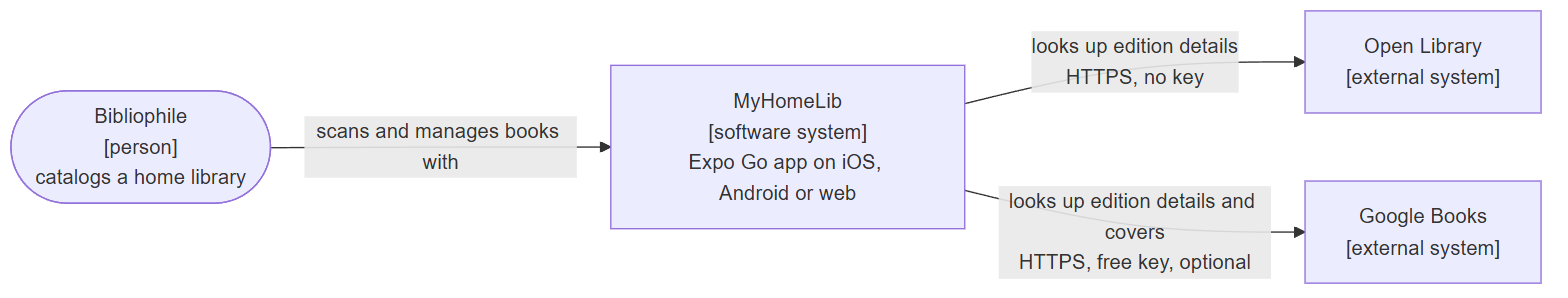
\includegraphics[width=0.85\textwidth, height=0.22\textheight, keepaspectratio]{figures/context.png}
\caption{C4 Level 1 -- System Context}
\label{fig:context}
\end{figure}

Figure~\ref{fig:context} shows MyHomeLib in its environment. A single type of user, the bibliophile, catalogs books with the app. The app depends on two external systems for book metadata: Open Library, which needs no key, and Google Books, which is optional and needs a free API key. Everything else runs on the user's device.

\begin{figure}[htbp]
\centering
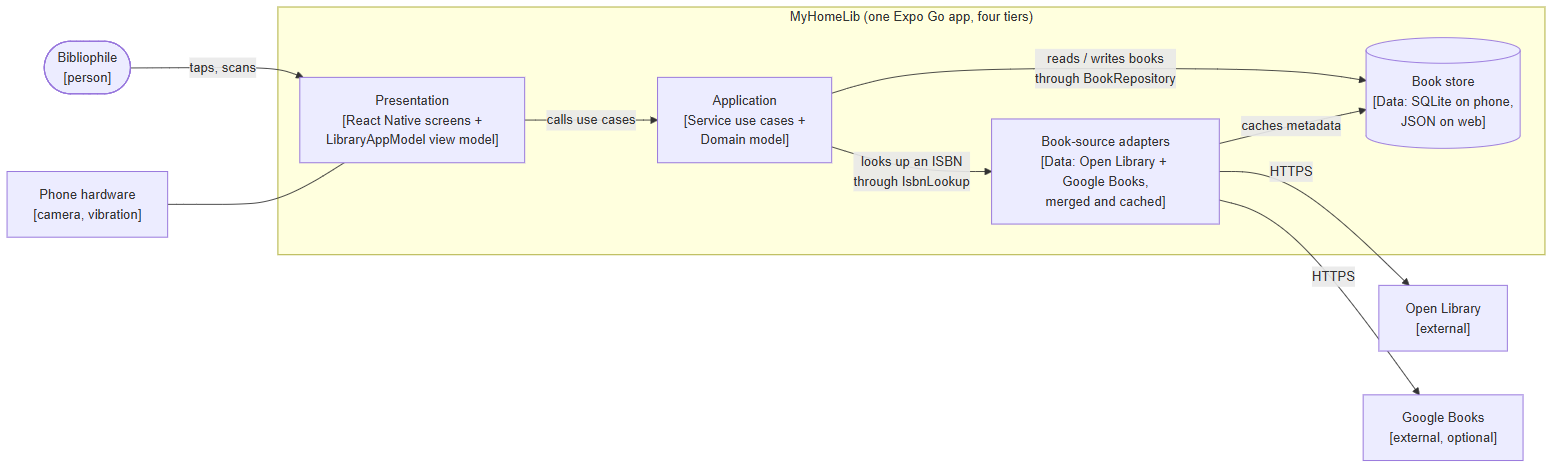
\includegraphics[width=\textwidth, height=0.36\textheight, keepaspectratio]{figures/system-overview.png}
\caption{C4 Level 2 -- Container (System Architecture)}
\label{fig:system_architecture}
\end{figure}

Figure~\ref{fig:system_architecture} shows the architecture chosen for MyHomeLib: a \textbf{four-tier modular monolith} in one TypeScript codebase. The tiers are folders with a strict dependency direction, enforced by automated tests:

\begin{itemize}
    \item \textbf{Presentation} (\texttt{presentation/}): React Native screens rendered by Expo, and the \texttt{LibraryAppModel} view model that holds all screen state and user flows. Components only render and forward taps.
    \item \textbf{Service} (\texttt{service/}): one class per use case (scan a book, move a book, set reading status, and so on) plus the \emph{ports}, the interfaces that the Data tier implements.
    \item \textbf{Domain} (\texttt{domain/}): the business objects and rules: \texttt{Book}, \texttt{PersonalLibrary}, and the acquisition records \texttt{Purchase} and \texttt{Gift}. Domain imports nothing outside itself.
    \item \textbf{Data} (\texttt{data/}): the adapters to the outside world: SQLite on a phone, browser storage on the web, and the Open Library and Google Books lookups, merged and cached.
\end{itemize}

Calls always flow Presentation $\rightarrow$ Service $\rightarrow$ Domain and ports, never backwards. The Data tier depends on the Service ports, not the other way around, so the business rules can be tested with in-memory fakes and the storage technology can change without touching them. A composition root (\texttt{bootstrap.ts}) is the only place that chooses concrete adapters and wires them into the use cases.

Because MyHomeLib runs in Expo Go, the same code reaches iOS, Android, and the web. The architecture can be extended with cloud synchronization or a second user by adding a new repository adapter behind the same port; this is out of scope for this version.

%==========================================================================
\section{System Components}
\label{sec:components}

\subsection{Decomposition Description}

\begin{figure}[htbp]
\centering
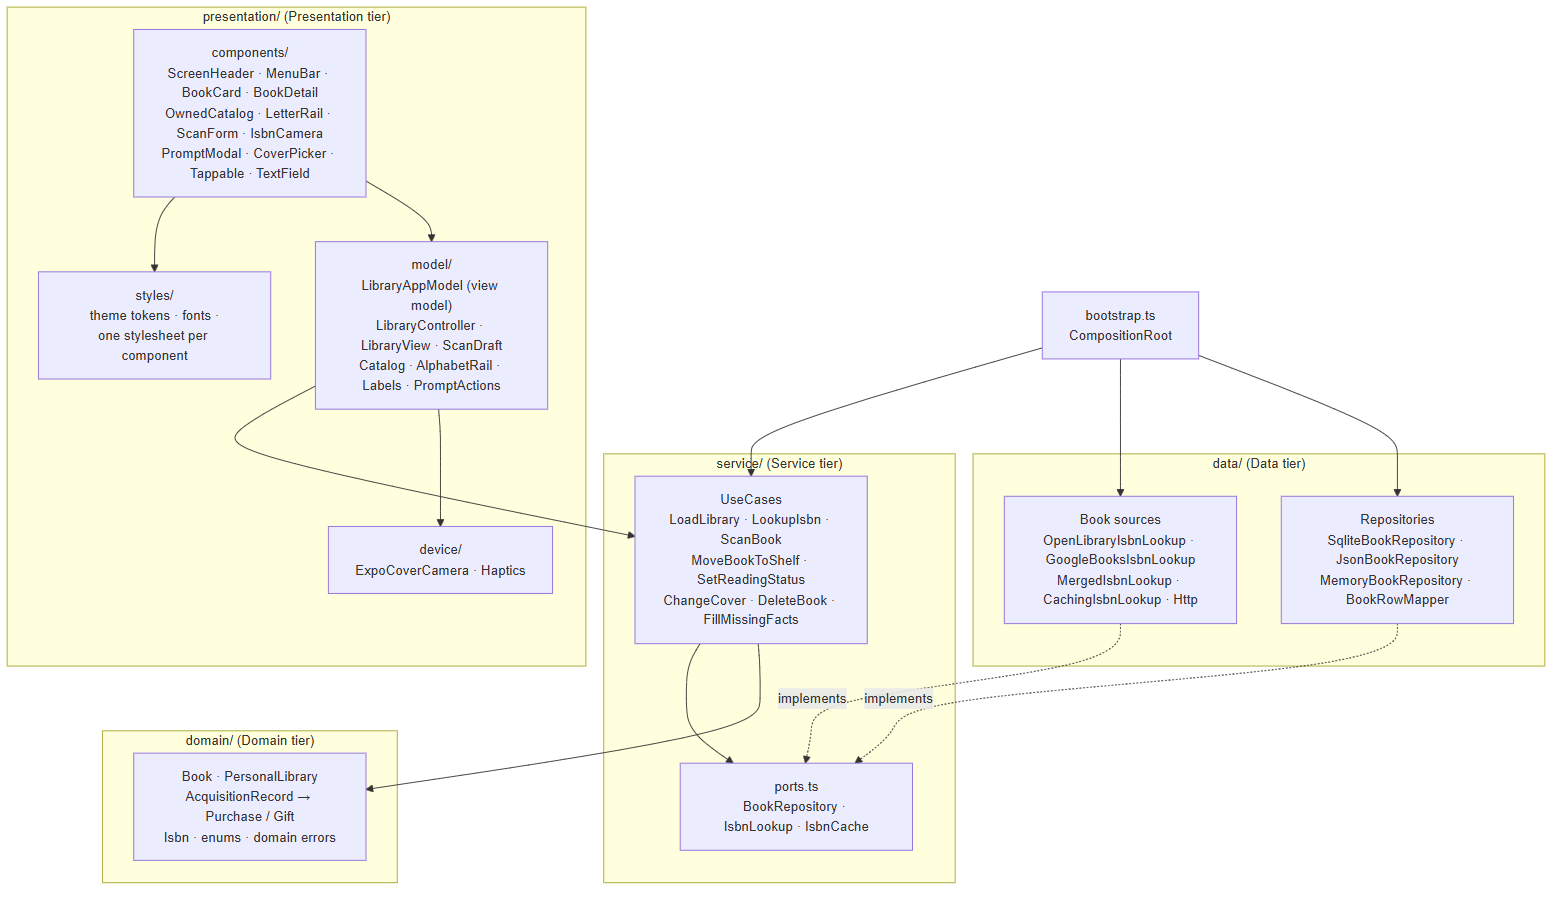
\includegraphics[width=\textwidth, height=0.5\textheight, keepaspectratio]{figures/decomposition.png}
\caption{System Decomposition Diagram (folders and their classes)}
\label{fig:decomposition}
\end{figure}

Figure~\ref{fig:decomposition} shows a top-down decomposition of the codebase. Each tier is a folder, and each folder holds classes with one responsibility each:

The \textbf{Presentation view model} (\texttt{presentation/model/}) is the controller of the C4 component view. \texttt{LibraryAppModel} extends a reusable \texttt{Observable} base class and holds every screen's state: the selected tab, the open popup, the scan draft, and the flash message. \texttt{LibraryController} turns screen intents into use case calls and returns a \texttt{LibraryView} snapshot. Helper classes keep logic out of the views: \texttt{ScanDraft} (a scan in progress), \texttt{Catalog} and its grouping strategies, \texttt{AlphabetRail} (letter-rail math), \texttt{Labels} (all display wording), and \texttt{PromptActions} (popup buttons).

The \textbf{Presentation views} (\texttt{presentation/components/} and \texttt{presentation/styles/}) are React components that only render. Every component imports its stylesheet from \texttt{styles/}, and every color, size, and font comes from the theme tokens. Shared building blocks (\texttt{Tappable}, \texttt{TextField}, \texttt{BookCover}, \texttt{CoverBackdrop}, \texttt{Logo}, \texttt{Reveal}) replace repeated code.

The \textbf{Device adapters} (\texttt{presentation/device/}) wrap phone hardware: \texttt{ExpoCoverCamera} implements the \texttt{CoverCamera} interface for cover photos, and \texttt{Haptics} gives physical feedback.

The \textbf{Service use cases} (\texttt{service/}) orchestrate one user goal each. Eight use case classes are built once by the \texttt{UseCases} class from two ports.

The \textbf{Domain model} (\texttt{domain/}) enforces the collection rules. Its state is private and changes only through methods that check the rules.

The \textbf{Book repositories} (\texttt{data/}) persist the library: \texttt{SqliteBookRepository} on a phone, \texttt{JsonBookRepository} on the web, and \texttt{MemoryBookRepository} for tests, all translating rows through \texttt{BookRowMapper}.

The \textbf{Book-source adapters} (\texttt{data/}) look up an ISBN: \texttt{OpenLibraryIsbnLookup} and \texttt{GoogleBooksIsbnLookup}, combined by \texttt{MergedIsbnLookup} and cached by \texttt{CachingIsbnLookup}. All HTTP goes through one \texttt{Http} class.

\subsection{Dependency Description}

\begin{figure}[htbp]
\centering
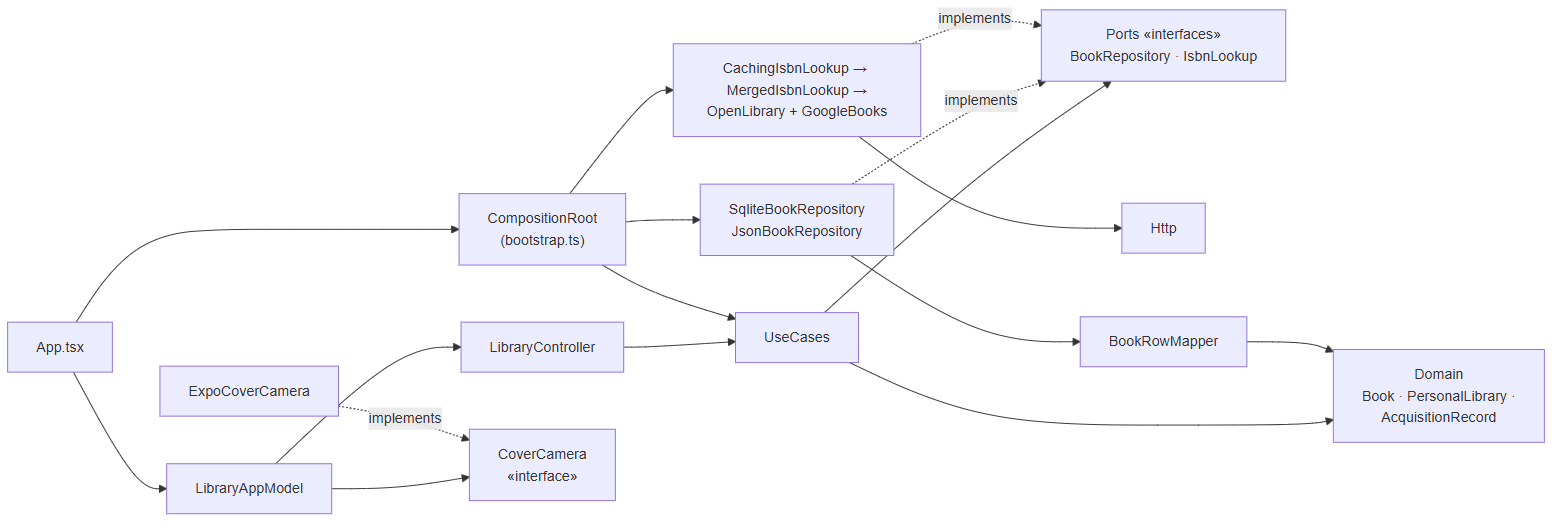
\includegraphics[width=\textwidth, height=0.36\textheight, keepaspectratio]{figures/dependency.png}
\caption{System Dependency Diagram}
\label{fig:dependency}
\end{figure}

Figure~\ref{fig:dependency} shows how each module depends on the others. \texttt{App.tsx} creates the \texttt{LibraryAppModel}, which uses \texttt{LibraryController} to reach the \texttt{UseCases}. The use cases depend on the Domain classes and on two \emph{interfaces}, \texttt{BookRepository} and \texttt{IsbnLookup}. The concrete repositories and lookups depend on those interfaces (they implement them), which inverts the usual direction: Service never imports Data (the Dependency Inversion Principle, ADR-009).

\texttt{CompositionRoot} in \texttt{bootstrap.ts} is the only module that knows every concrete class. At start-up it opens SQLite (or browser storage when SQLite is unavailable), wraps the merged book sources in the cache, and hands the finished \texttt{UseCases} to the view model. The camera follows the same idea one tier up: the view model depends on the \texttt{CoverCamera} interface, and the app passes \texttt{ExpoCoverCamera} while tests pass a fake.

These rules are not only documented; \texttt{tests/architecture.test.ts} reads every source file and fails if Domain imports anything outside Domain, if Service imports Data or calls \texttt{fetch}, if Data imports Presentation or React, if Presentation reaches a repository, if a component defines its own stylesheet, or if any file other than \texttt{App.tsx} reaches the composition root.

\subsection{Interface Description}

\subsubsection{Presentation View Model}

\begin{figure}[htbp]
\centering
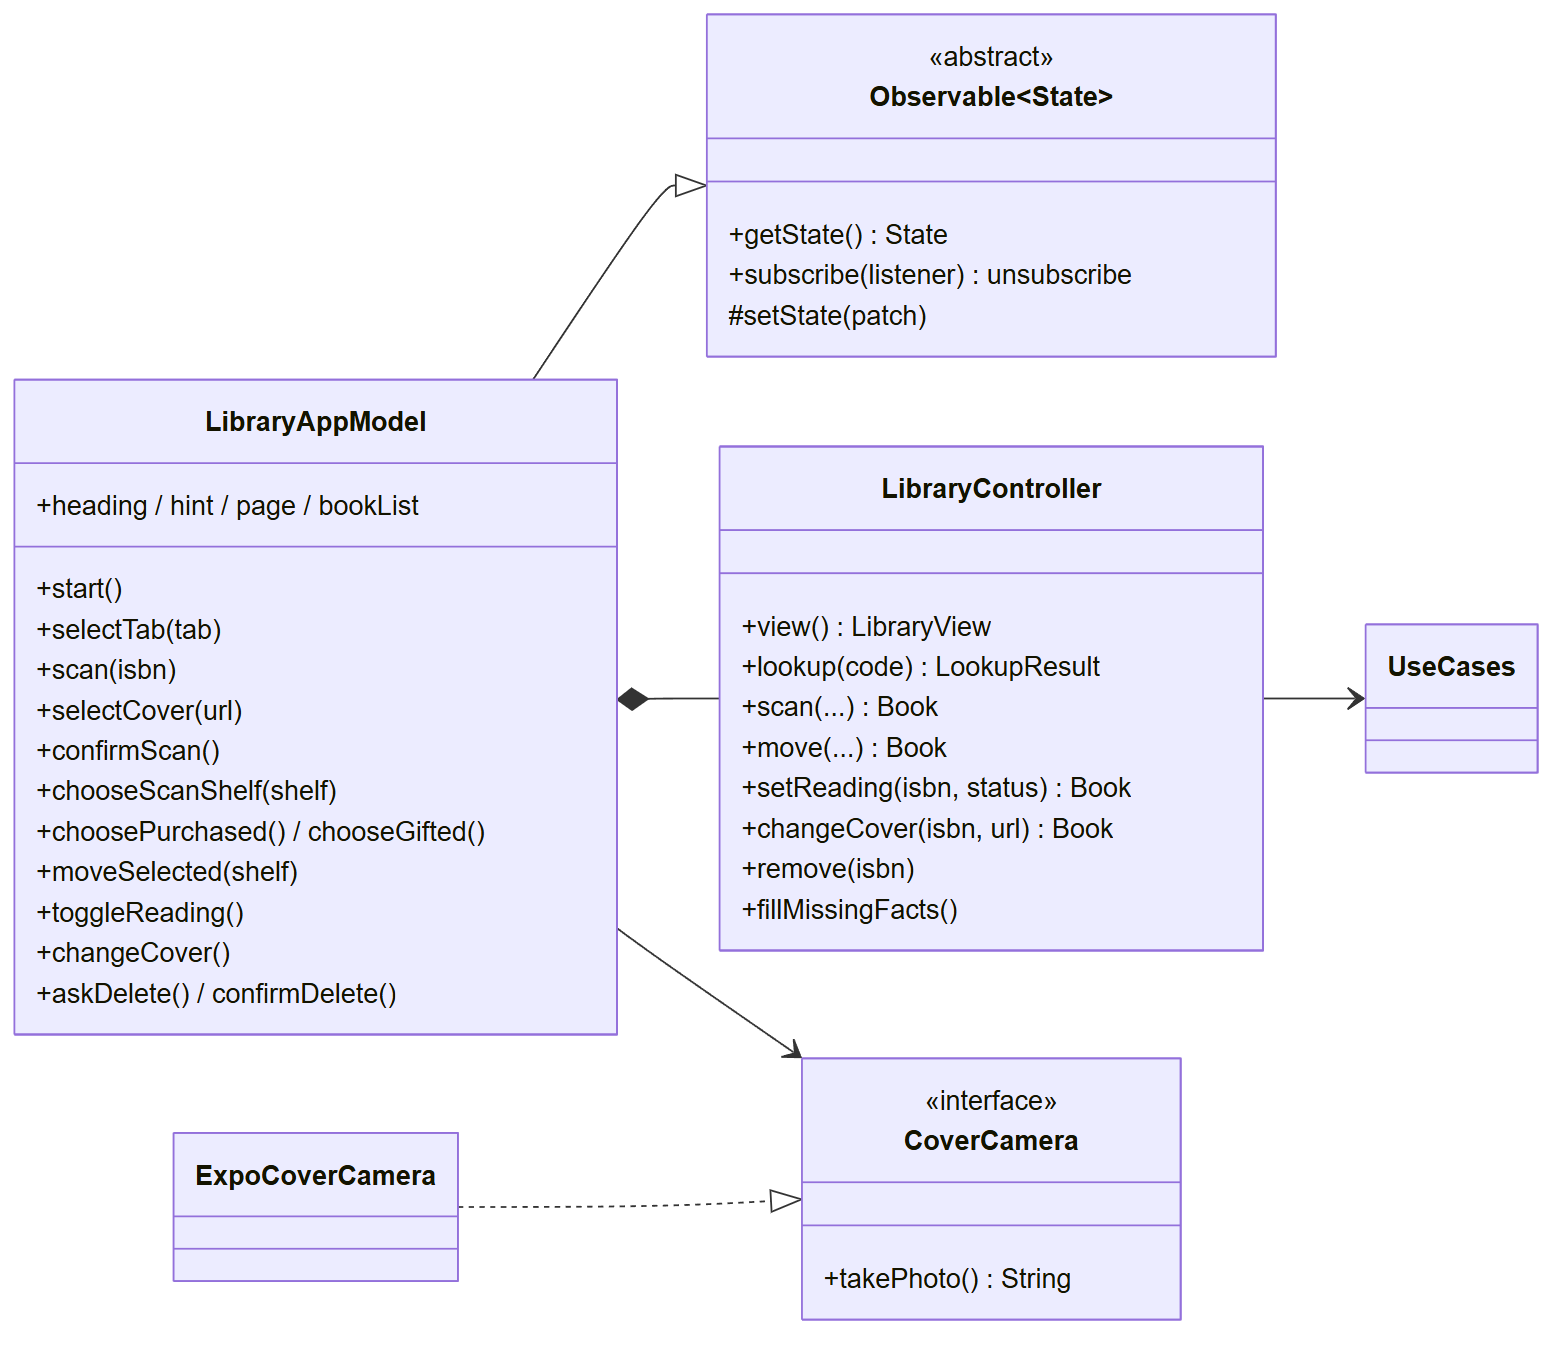
\includegraphics[width=\textwidth, height=0.48\textheight, keepaspectratio]{figures/iface-presentation.png}
\caption{Presentation View Model Interface}
\label{fig:iface_presentation}
\end{figure}

Figure~\ref{fig:iface_presentation} shows the interface between the screens and the rest of the app. Screens read \texttt{LibraryAppModel}'s state and derived values (\texttt{heading}, \texttt{hint}, \texttt{page}, \texttt{bookList}) and call its intent methods (\texttt{scan}, \texttt{confirmScan}, \texttt{chooseGifted}, \texttt{moveSelected}, \ldots). React subscribes through one hook, \texttt{useObservable}, so every state change re-renders the screens. The model calls the use cases only through \texttt{LibraryController}, and takes cover photos only through the \texttt{CoverCamera} interface.

\subsubsection{Service Use Cases}

\begin{figure}[htbp]
\centering
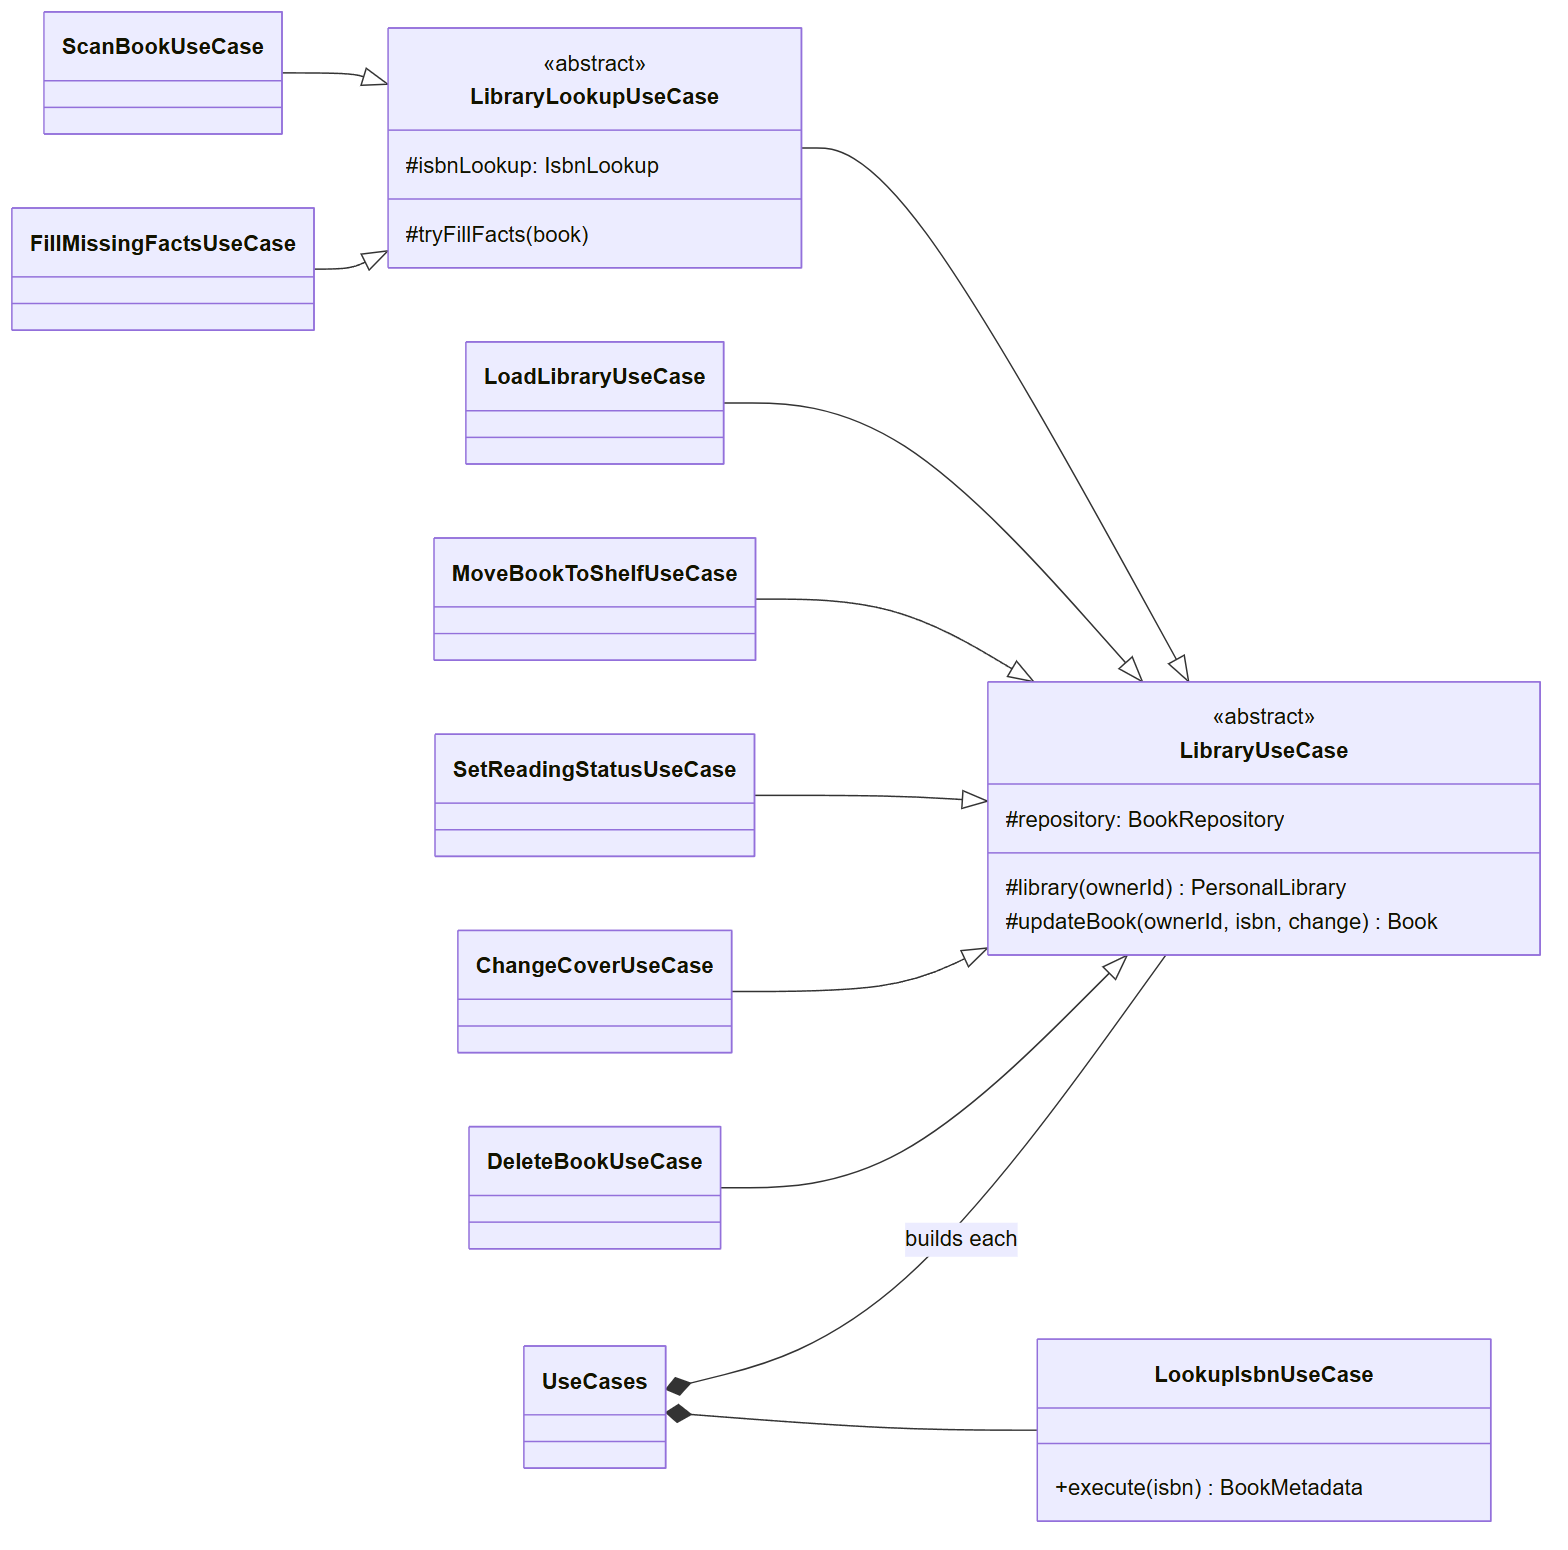
\includegraphics[width=\textwidth, height=0.42\textheight, keepaspectratio]{figures/iface-service.png}
\caption{Service Use Case Interface}
\label{fig:iface_service}
\end{figure}

Figure~\ref{fig:iface_service} shows the use case classes. Every library use case extends the abstract \texttt{LibraryUseCase}, which implements the shared load $\rightarrow$ change $\rightarrow$ save steps once (\texttt{updateBook}, a Template Method). Use cases that also need the book sources extend \texttt{LibraryLookupUseCase}. \texttt{LookupIsbnUseCase} only reads, so it stands alone. Each use case exposes a single \texttt{execute(...)} method.

\subsubsection{Domain Model}

\begin{figure}[htbp]
\centering
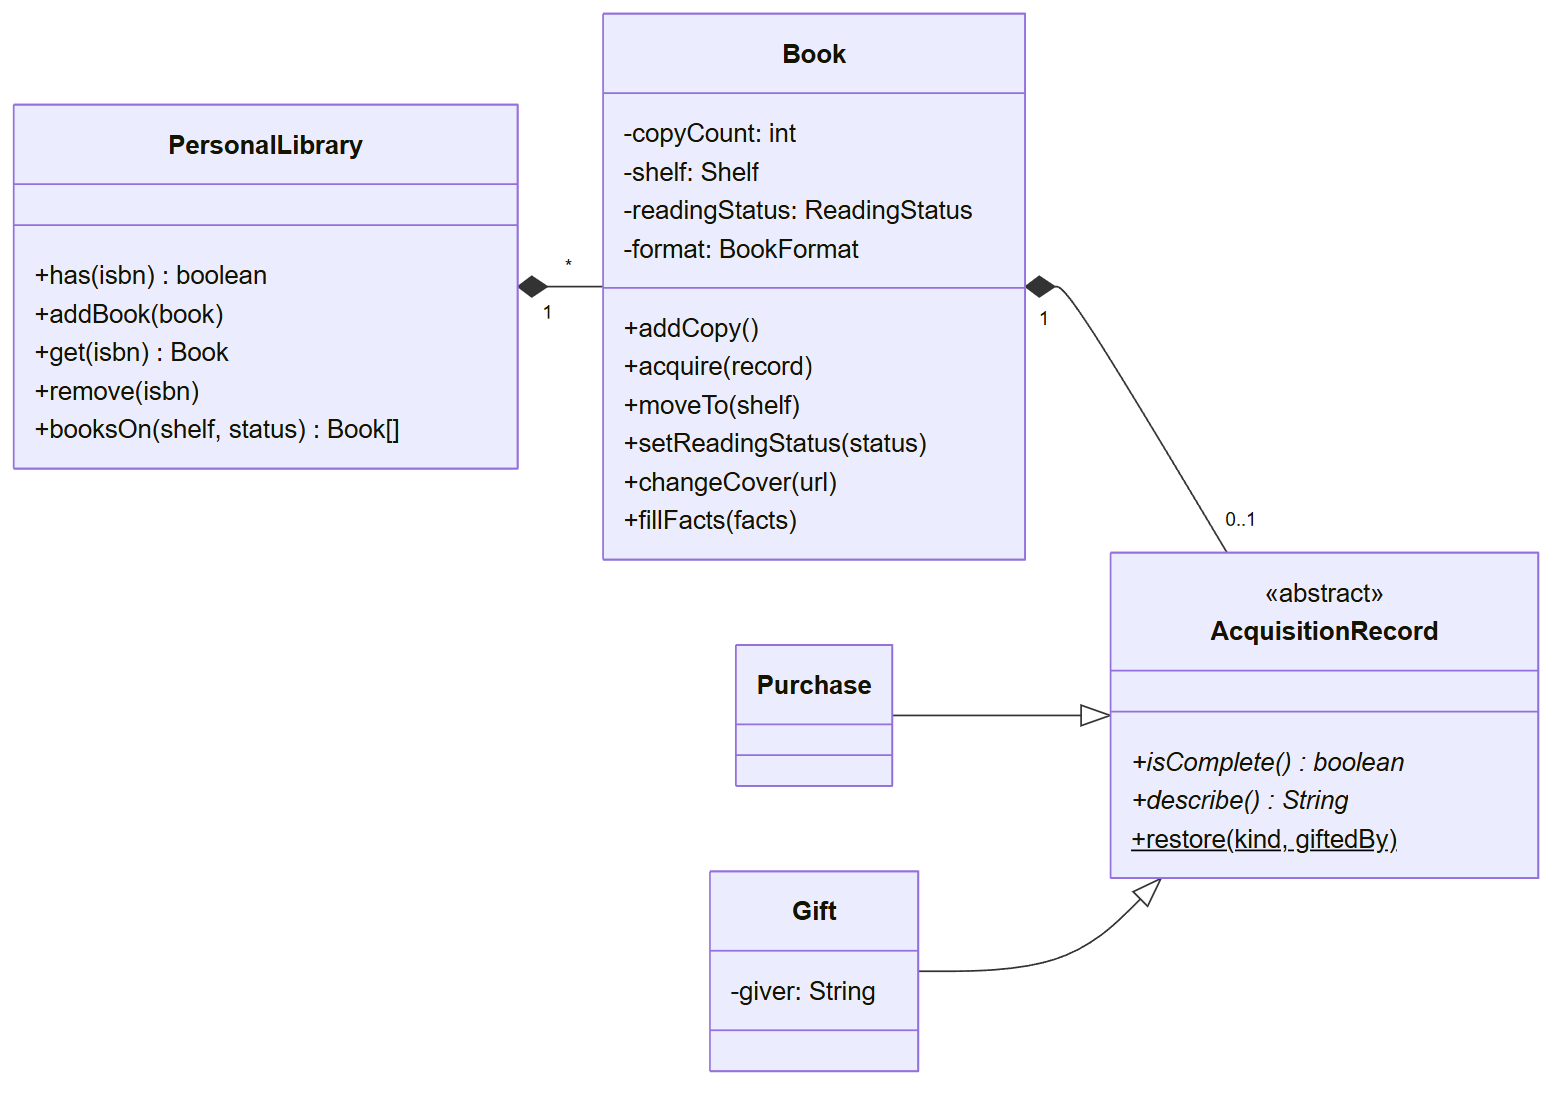
\includegraphics[width=\textwidth, height=0.36\textheight, keepaspectratio]{figures/iface-domain.png}
\caption{Domain Model Interface}
\label{fig:iface_domain}
\end{figure}

Figure~\ref{fig:iface_domain} shows the domain interface. \texttt{PersonalLibrary} composes the \texttt{Book} objects of one owner. \texttt{Book} keeps its fields private and offers intention-revealing methods (\texttt{addCopy}, \texttt{acquire}, \texttt{moveTo}, \ldots) that throw a domain error when a rule is broken. \texttt{AcquisitionRecord} is abstract; \texttt{Purchase} and \texttt{Gift} implement \texttt{isComplete()} and \texttt{describe()} polymorphically, so \texttt{Book} never branches on the acquisition type.

\subsubsection{Book Repositories}

\begin{figure}[htbp]
\centering
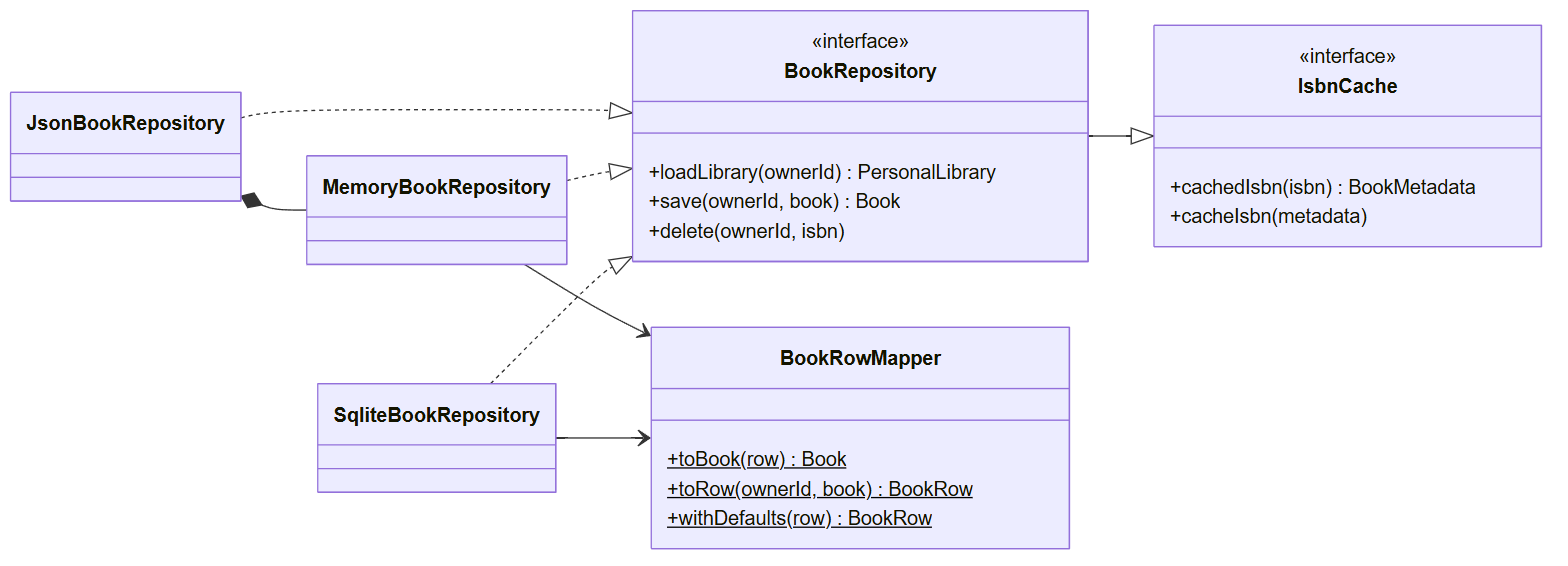
\includegraphics[width=0.9\textwidth, height=0.3\textheight, keepaspectratio]{figures/iface-data.png}
\caption{Book Repository Interface}
\label{fig:iface_data}
\end{figure}

Figure~\ref{fig:iface_data} shows the persistence interface. \texttt{BookRepository} extends \texttt{IsbnCache}, so one store holds both the library and the cached lookups. Three adapters implement it. \texttt{JsonBookRepository} reuses \texttt{MemoryBookRepository} by composition and only adds loading and saving to browser storage. \texttt{BookRowMapper} is the single translation between a stored row and a \texttt{Book} (Data Mapper pattern), including the defaults for rows saved by older versions.

\subsubsection{Book-Source Adapters}

\begin{figure}[htbp]
\centering
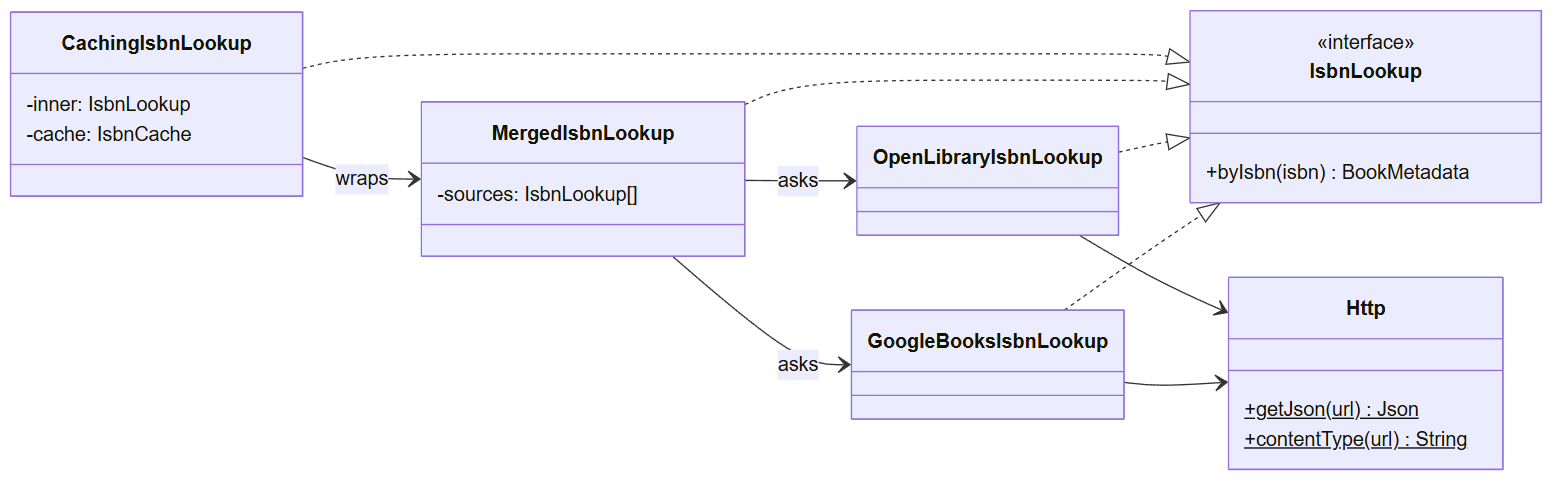
\includegraphics[width=\textwidth, height=0.3\textheight, keepaspectratio]{figures/iface-sources.png}
\caption{Book-Source Adapter Interface}
\label{fig:iface_sources}
\end{figure}

Figure~\ref{fig:iface_sources} shows the lookup chain. Every element implements the same \texttt{IsbnLookup} interface, so they stack as decorators: \texttt{CachingIsbnLookup} answers from the cache or asks \texttt{MergedIsbnLookup}, which asks Google Books and Open Library together, merges the answers field by field (edition data first), and keeps every distinct cover as a candidate. Both sources reach the network only through the \texttt{Http} class.

\subsubsection{Device Adapters}

The camera and the vibration motor are wrapped so that the view model never touches device APIs directly. \texttt{ExpoCoverCamera} implements \texttt{CoverCamera}: it opens the camera, lets the owner crop to the cover, and shrinks the photo to a small JPEG stored with the book. \texttt{Haptics} gives a light tick when a tab changes, a soft tap for a message, and a buzz for an error, and does nothing on the web. The ISBN barcode scanner is \texttt{IsbnCamera}, a view that reports each new code to the view model.

\subsection{Module Interfaces}

The following TypeScript interfaces are the contracts between tiers. The Service tier owns them (\texttt{service/ports.ts}); the Data tier implements them.

\begin{lstlisting}
/** What the book sources know about one ISBN (one edition). */
export type BookMetadata = BookFacts & {
  isbn: string; title: string; author: string; publisher: string;
  coverUrl: string;            // best cover first
  coverCandidates: string[];   // every distinct cover the sources offer
};

export interface IsbnLookup {
  byIsbn(isbn: string): Promise<BookMetadata>;
}

export interface IsbnCache {
  cachedIsbn(isbn: string): Promise<BookMetadata | null>;
  cacheIsbn(metadata: BookMetadata): Promise<void>;
}

export interface BookRepository extends IsbnCache {
  loadLibrary(ownerId: string): Promise<PersonalLibrary>;
  save(ownerId: string, book: Book): Promise<Book>;
  delete(ownerId: string, isbn: string): Promise<void>;
}
\end{lstlisting}

The Presentation tier owns two more contracts: the device camera, and the reusable observable base class of the view model.

\begin{lstlisting}
export interface CoverCamera {
  // A small image of the cover (data URI), or null if the owner backed out.
  takePhoto(): Promise<string | null>;
}

export abstract class Observable<State> {
  getState(): State;
  subscribe(listener: () => void): () => void;   // returns unsubscribe
  protected setState(patch: Partial<State>): void;
}
\end{lstlisting}

\subsection{User Interfaces (GUI)}

The interface uses one design system: a dark ``enchanted forest'' background, a single mint accent reserved for selection and primary actions, the Outfit typeface in four weights, and a floating tab dock with TBR, Owned, Wanted, and Scan. All screenshots below were captured from the running application at phone size.

\subsubsection{To Be Read}

\begin{figure}[htbp]
\centering
\screen{tbr-unread}\hfill\screen{tbr-read}\hfill\screen{empty-tbr}
\caption{To be read: Unread (left), Read (center), and the empty state (right)}
\label{fig:gui_tbr}
\end{figure}

Figure~\ref{fig:gui_tbr} shows the TBR screen, the app's home. The switch at the top splits Owned books into Unread and Read, with a count on each side. Each card shows the cover, title, author, binding, and copy count; a leaf marks books already read. An empty shelf explains itself and offers a Scan button.

\subsubsection{Owned Catalog}

\begin{figure}[htbp]
\centering
\screen{owned-az}\hfill\screen{owned-author}\hfill\screen{owned-series-expanded}
\caption{Owned catalog grouped A--Z (left), by author (center), and by series (right)}
\label{fig:gui_owned}
\end{figure}

Figure~\ref{fig:gui_owned} shows the full Owned catalog. The switch chooses the grouping; each section starts with an index heading. In the series grouping, a series appears as a fan of its covers with a count badge, and tapping it expands its books. The A--Z rail on the right jumps to a section when tapped or dragged.

\subsubsection{Wanted}

\begin{figure}[htbp]
\centering
\screen{wanted}\hspace{1cm}\screen{detail-wanted}
\caption{Wanted list (left) and a Wanted book's detail (right)}
\label{fig:gui_wanted}
\end{figure}

Figure~\ref{fig:gui_wanted} shows the wish list. A Wanted book has the same detail screen as an Owned one, with a ``To Owned'' action instead of ``To Wanted''.

\subsubsection{Scan}

\begin{figure}[htbp]
\centering
\screen{scan}\hfill\screen{scan-confirm}\hfill\screen{scan-shelf}
\caption{Scan screen (left), the confirm popup with the cover picker (center), and the shelf choice (right)}
\label{fig:gui_scan}
\end{figure}

Figure~\ref{fig:gui_scan} shows the scan flow. The camera reads the barcode inside the corner brackets; the ISBN can also be typed. The confirm popup shows the edition's details and every cover the sources offer, on a soft halo of the selected cover, plus a ``Your photo'' tile. Nothing is saved until the owner has answered every question.

\subsubsection{Book Detail}

\begin{figure}[htbp]
\centering
\screen{detail-top}\hspace{1cm}\screen{detail-actions}
\caption{Book detail: cover and facts (left), description and actions (right)}
\label{fig:gui_detail}
\end{figure}

Figure~\ref{fig:gui_detail} shows a book's detail screen: the cover on a halo of its own colors, status tags, the edition's facts (publisher, date, pages, series, ISBN, copies, and how it was acquired), the description and subjects, and the actions: mark read or unread, move between shelves, replace the cover with a photo, and delete.

%==========================================================================
\section{Detailed Design}

\textbf{Sequence Diagrams}

\begin{figure}[htbp]
    \centering
    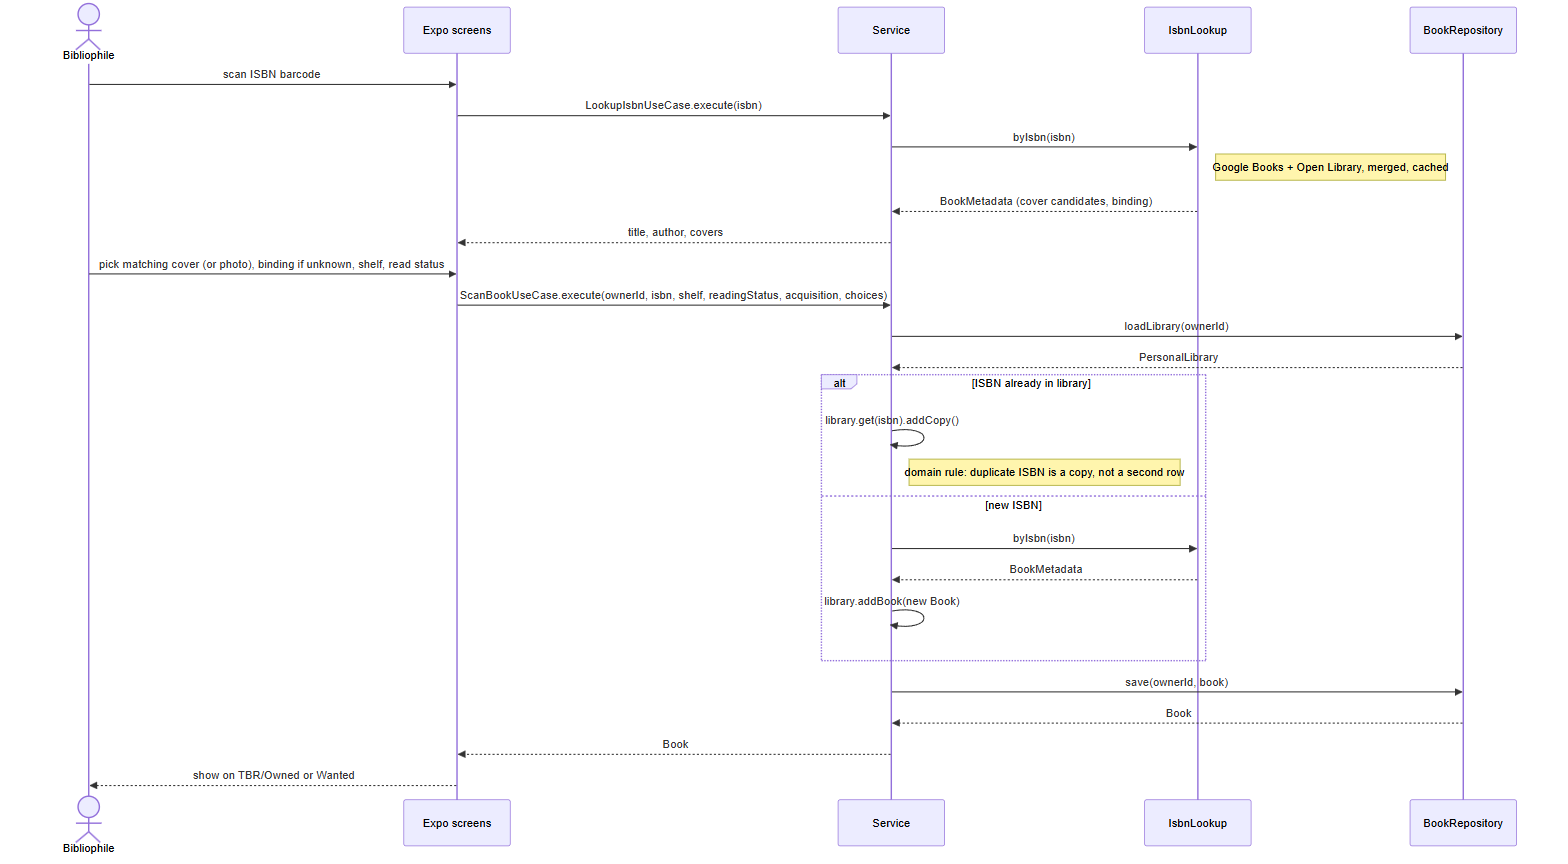
\includegraphics[width=\textwidth, height=0.6\textheight, keepaspectratio]{figures/sequence-scan.png}
    \caption{Sequence diagram: scanning a book (lookup, confirm, save)}
    \label{fig:sequence_scan}
\end{figure}

Figure~\ref{fig:sequence_scan} shows the main use case. The lookup saves nothing; it returns the edition's details and cover candidates. Only after the owner confirms does \texttt{ScanBookUseCase} load the library, add a copy or a new \texttt{Book}, and save it.

\begin{figure}[htbp]
    \centering
    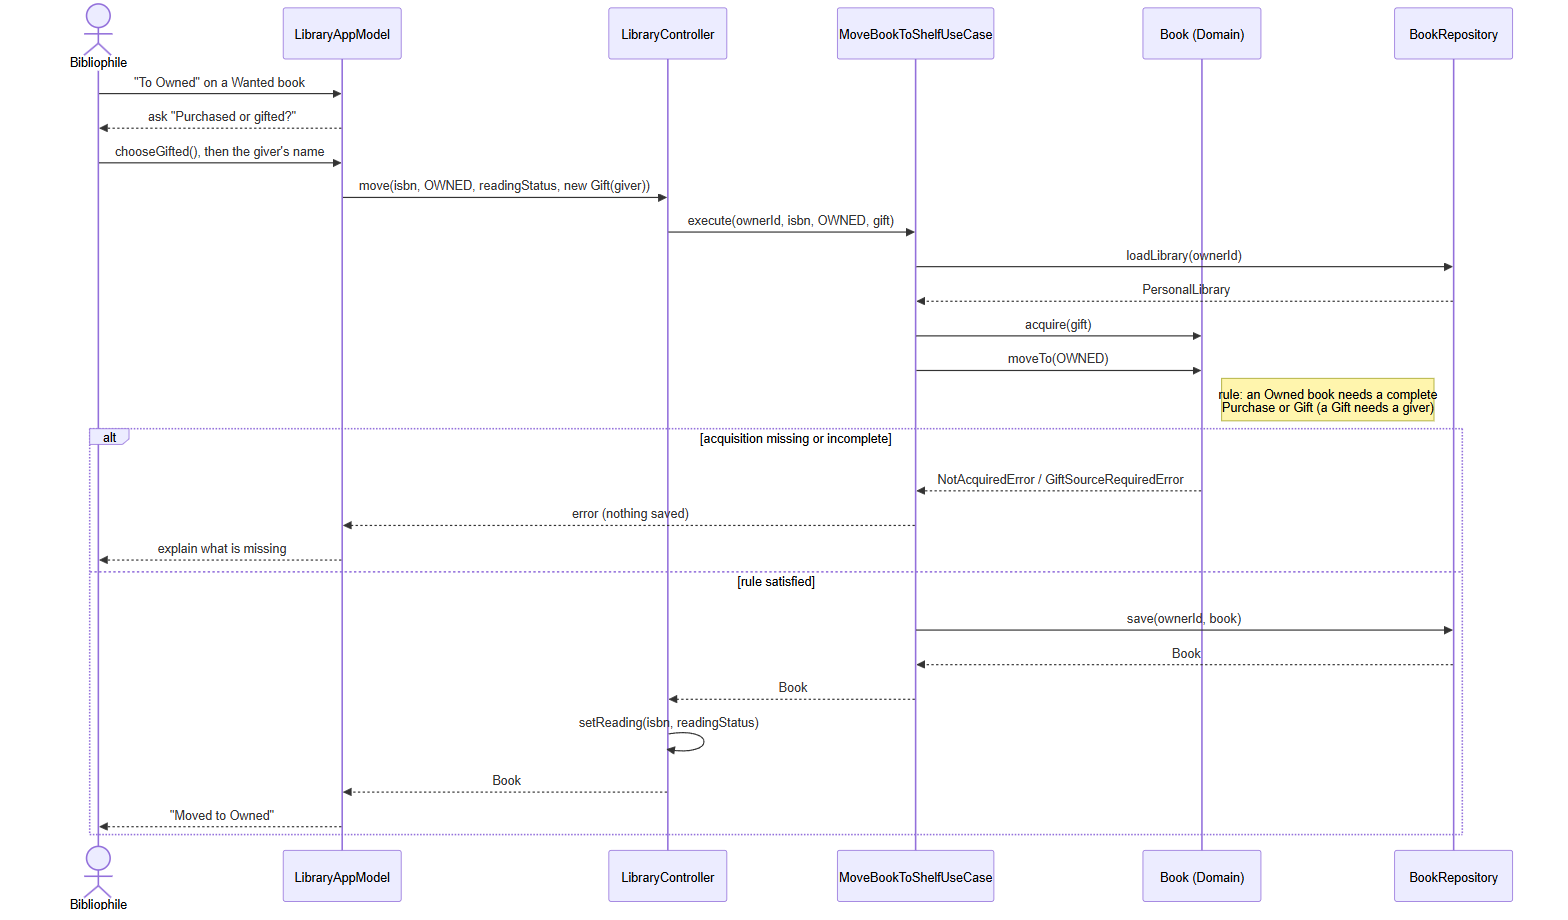
\includegraphics[width=\textwidth, height=0.52\textheight, keepaspectratio]{figures/sequence-move.png}
    \caption{Sequence diagram: moving a Wanted book to Owned as a gift}
    \label{fig:sequence_move}
\end{figure}

Figure~\ref{fig:sequence_move} shows how a domain rule is enforced. The view model gathers the acquisition first; \texttt{Book.moveTo} then refuses to move a book to Owned without a complete \texttt{Purchase} or \texttt{Gift}, and nothing is saved when the rule fails.

\textbf{Pseudocode (scan a book)}

\begin{verbatim}
User opens Scan
If camera permission granted:
    Read the ISBN barcode from the camera preview
Else:
    User types the ISBN
metadata = cache.get(isbn) or merge(GoogleBooks(isbn), OpenLibrary(isbn))
If no source knows the ISBN:
    Show "No book found for ISBN ..."; stop
Show the edition and its cover candidates
If the ISBN is already in the library:
    On confirm: book.addCopy(); save(book); stop
Owner picks the cover that matches their copy (or photographs it)
If the binding is unknown:
    Ask "Hardcover or paperback?"
Ask "Owned or Wanted?"
If Owned:
    Ask "Purchased or gifted?"
    If gifted: ask for the giver's name (required)
Ask "Read or unread?"
library.addBook(new Book(metadata, choices))   // domain rules checked here
save(book); cache(metadata)
Show the book on TBR / Owned or Wanted
\end{verbatim}

\subsection{Data Detailed Design}

\begin{figure}[htbp]
\centering
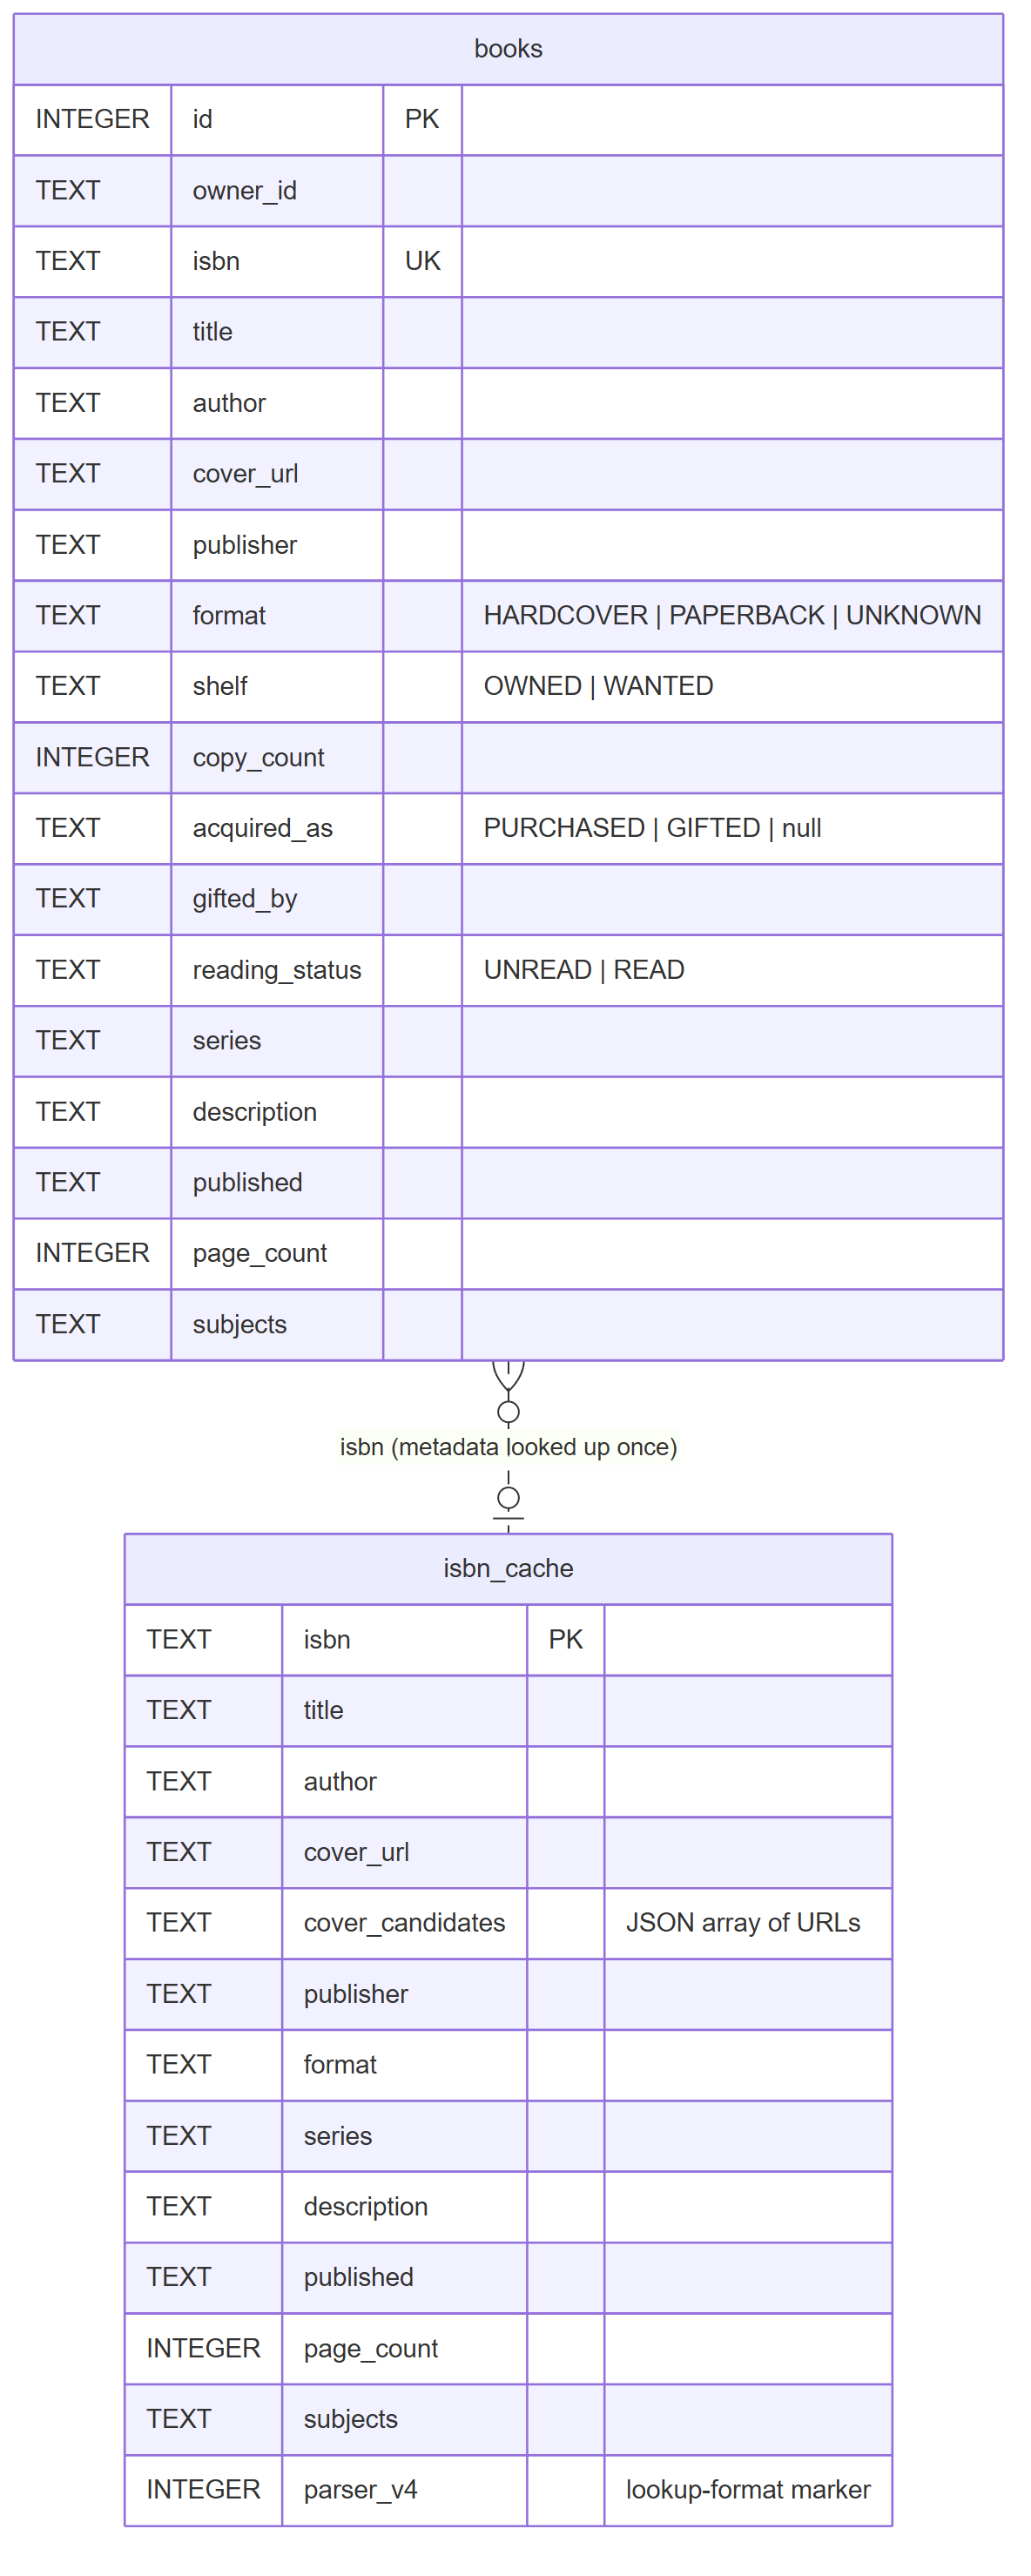
\includegraphics[width=0.6\textwidth, height=0.62\textheight, keepaspectratio]{figures/data-model.png}
\caption{Local data model (SQLite)}
\label{fig:data_model}
\end{figure}

Figure~\ref{fig:data_model} shows the two tables the app stores on the device. On the web the same data is kept as JSON in browser storage with the same field names.

\begin{itemize}
    \item \textbf{books}: one row per cataloged title and owner: the edition facts (title, author, publisher, date, pages, series, subjects, description), the chosen cover (a URL or an inline photo), the binding, the shelf, the copy count, the reading status, and the acquisition (\texttt{PURCHASED} or \texttt{GIFTED} with the giver's name). The ISBN is unique, which backs the ``duplicate ISBN adds a copy'' rule.
    \item \textbf{isbn\_cache}: one row per looked-up ISBN with the merged metadata and every cover candidate (as a JSON array), so a book is fetched from the network only once. A version marker clears old entries when the lookup format changes.
\end{itemize}

The schema migrates itself: missing columns are added when the app starts, and rows saved by older builds (for example the former third ``TBR'' shelf, now Owned and unread) are upgraded by \texttt{BookRowMapper}.

\subsection{RTM}

The Requirements Traceability Matrix links each requirement to the components that implement it and to the verification cases in Section~\ref{sec:verification}.

\begin{longtable}{|L{1.6cm}|L{5.2cm}|L{4.6cm}|L{2.6cm}|}
\hline
\textbf{Req.-ID} & \textbf{Requirement Description} & \textbf{Design Component} & \textbf{Test-Case \#} \\
\hline
\endhead
FR-1 & Scan an ISBN with the camera, or type it & IsbnCamera, ScanForm, LibraryAppModel & 15, 16, 21 \\ \hline
FR-2 & Look up the exact edition from Open Library and Google Books & OpenLibraryIsbnLookup, GoogleBooksIsbnLookup, MergedIsbnLookup & 16, 21, 22 \\ \hline
FR-3 & Pick the matching cover or photograph your own & CoverPicker, ScanDraft, CoverCamera & 17, 23 \\ \hline
FR-4 & Ask for the binding only when no source knows it & ScanDraft, LibraryAppModel & 18 \\ \hline
FR-5 & Shelve a scanned book as Owned or Wanted & ScanBookUseCase, PersonalLibrary & 14, 19 \\ \hline
FR-6 & An Owned book must be purchased or gifted; a gift needs the giver's name & Book, AcquisitionRecord, Purchase, Gift & 10--14 \\ \hline
FR-7 & A duplicate ISBN adds a copy instead of a second entry & Book.addCopy, ScanBookUseCase & 8 \\ \hline
FR-8 & Reading status is independent of the shelf; TBR shows Owned unread/read & Book, LibraryView, SetReadingStatusUseCase & 4, 5, 24 \\ \hline
FR-9 & Browse Owned A--Z, by author, or by series with a letter rail & Catalog, CatalogGrouping strategies, AlphabetRail & 6, 7 \\ \hline
FR-10 & Move a book between shelves & MoveBookToShelf\-UseCase, Book.moveTo & 10--13 \\ \hline
FR-11 & Delete a book only after confirmation & DeleteBookUseCase, LibraryAppModel & 25 \\ \hline
FR-12 & Cancel any popup without changing the library & LibraryAppModel\allowbreak.cancelPrompt & 20 \\ \hline
FR-13 & Persist the library and cache lookups on the device & SqliteBookRepository, JsonBookRepository, CachingIsbnLookup & 9 \\ \hline
NFR-1 & Tiers depend only downward; Service never imports Data & Ports, CompositionRoot, architecture tests & 26 \\ \hline
NFR-2 & Stylesheets are imports; values come from theme tokens & presentation/styles, architecture tests & 26 \\ \hline
NFR-3 & Runs in Expo Go (iOS, Android) and on the web without native builds & Expo modules only (ADR-005, ADR-008) & 27 \\ \hline
NFR-4 & Accessible: WCAG AA contrast, screen-reader labels, reduced motion & Theme tokens, Tappable, Reveal, Labels & 28 \\ \hline
NFR-5 & The architecture is documented: tier table, C4 and UML diagrams, ADRs & README, docs/adr, this SDD & 1--3 \\ \hline
\end{longtable}

%==========================================================================
\section{Sprint Planning}

MyHomeLib is an individual project, so every development role below is held by the same developer, with a peer review partner reviewing the work at the midterm and final sessions (October 12 and 19, and November 9 and 16). Work is organized as weekly sprints that follow the course milestones. The \emph{Proposed Timeline} below is the plan at project approval; the \emph{Actual Timeline} records what was built. The sprint dates stayed in the same calendar windows, but the content of two sprints changed. In proposed Sprint 5, the Wanted list was to include a bookstore price check by scraping retailer pages; the instructor asked for scraping to be removed (ADR-004), so actual Sprint 5 concentrated on the acquisition rules for moving books to Owned. In proposed Sprint 6, the plan was polish and testing; testing showed that Open Library alone often returned the wrong cover for a specific printing, so actual Sprint 6 added exact-edition lookup with Google Books (ADR-006), and refactored the code into classes with a view model and a design system (ADR-007, ADR-008) to meet the course's object-oriented requirements. Sprints 7--9 have not started yet and follow the proposed timeline.

\setlist[enumerate]{topsep=0pt, partopsep=0pt, parsep=0pt, itemsep=2pt, leftmargin=1.5em}

\subsection{Role Focuses}

\vspace{0.3em}

\noindent
\begin{tabular}{|L{3.4cm}|L{4.2cm}|L{7.4cm}|}
\hline
\textbf{Team Member} & \textbf{Role} & \textbf{Responsibilities} \\
\hline
Grace Hechavarria & Architect, Developer, UI/UX Designer, Tester & Requirements and domain rules, architecture and ADRs, all four tiers, interface design, automated tests, and documentation \\
\hline
Yousef Habouh & Peer Review Partner & Runs the app from the README, compares the diagrams to the code, and files the structured midterm and final reviews \\
\hline
\end{tabular}

\subsection{Sprint Schedule, User Stories, and Acceptance Criteria}

\subsubsection{Proposed Timeline}

%%% PROPOSED SPRINT 1 %%%
\noindent\begin{minipage}{\linewidth}
\noindent{\textbf{\large Sprint 1 -- Project Proposal and Approval}}

\vspace{0.5em}
\noindent
\begin{tabular}{|L{1.2cm}|L{1.8cm}|L{5.2cm}|L{6.3cm}|}
\hline
\textbf{Sprint} & \textbf{Dates} & \textbf{User Stories} & \textbf{Acceptance Criteria} \\
\hline
Sprint 1 & 08/24 -- 08/30 &
As the instructor, I want a clear project idea and platform, so that I can approve the scope. &
\begin{enumerate}
    \item Verify that the repository exists with a README.
    \item Verify that the approval paragraph names the platform and the core features.
\end{enumerate} \\
\hline
\end{tabular}

\vspace{0.5em}
\noindent
\begin{tabular}{|L{3.4cm}|L{11.6cm}|}
\hline
\textbf{Team Member} & \textbf{Task} \\
\hline
Grace Hechavarria & Create the repository; draft project ideas; write the approval paragraph \\
\hline
\end{tabular}
\end{minipage}

\vspace{1.5em}

%%% PROPOSED SPRINT 2 %%%
\noindent\begin{minipage}{\linewidth}
\noindent{\textbf{\large Sprint 2 -- Tier Breakdown}}

\vspace{0.5em}
\noindent
\begin{tabular}{|L{1.2cm}|L{1.8cm}|L{5.2cm}|L{6.3cm}|}
\hline
\textbf{Sprint} & \textbf{Dates} & \textbf{User Stories} & \textbf{Acceptance Criteria} \\
\hline
Sprint 2 & 08/31 -- 09/06 &
As a developer, I want each tier's responsibilities written down, so that every class has an obvious home. &
\begin{enumerate}
    \item Verify that the README has a Presentation / Service / Domain / Data table.
    \item Verify that each row names the system's real responsibilities.
\end{enumerate} \\
\hline
\end{tabular}

\vspace{0.5em}
\noindent
\begin{tabular}{|L{3.4cm}|L{11.6cm}|}
\hline
\textbf{Team Member} & \textbf{Task} \\
\hline
Grace Hechavarria & Write the tier table for the README \\
\hline
\end{tabular}
\end{minipage}

\vspace{1.5em}

%%% PROPOSED SPRINT 3 %%%
\noindent\begin{minipage}{\linewidth}
\noindent{\textbf{\large Sprint 3 -- C4 and UML Models}}

\vspace{0.5em}
\noindent
\begin{tabular}{|L{1.2cm}|L{1.8cm}|L{5.2cm}|L{6.3cm}|}
\hline
\textbf{Sprint} & \textbf{Dates} & \textbf{User Stories} & \textbf{Acceptance Criteria} \\
\hline
Sprint 3 & 09/07 -- 09/20 &
As a reviewer, I want C4 and class diagrams, so that I can understand the system before reading code. &
\begin{enumerate}
    \item Verify that the README has C4 Context, Container, and Component diagrams.
    \item Verify that a UML class diagram shows the domain rules.
\end{enumerate} \\
\hline
\end{tabular}

\vspace{0.5em}
\noindent
\begin{tabular}{|L{3.4cm}|L{11.6cm}|}
\hline
\textbf{Team Member} & \textbf{Task} \\
\hline
Grace Hechavarria & Draw the C4 diagrams and the UML class diagram \\
\hline
\end{tabular}
\end{minipage}

\vspace{1.5em}

%%% PROPOSED SPRINT 4 %%%
\noindent\begin{minipage}{\linewidth}
\noindent{\textbf{\large Sprint 4 -- Scanning, Shelves, and Copies}}

\vspace{0.5em}
\noindent
\begin{tabular}{|L{1.2cm}|L{1.8cm}|L{5.2cm}|L{6.3cm}|}
\hline
\textbf{Sprint} & \textbf{Dates} & \textbf{User Stories} & \textbf{Acceptance Criteria} \\
\hline
Sprint 4 & 09/21 -- 09/27 &
As a bibliophile, I want to scan an ISBN and shelve the book as Owned or Wanted, so that I can build my catalog quickly. &
\begin{enumerate}
    \item Verify that an ISBN can be scanned or typed.
    \item Verify that a duplicate ISBN adds a copy.
    \item Verify that TBR lists Owned books by reading status.
\end{enumerate} \\
\hline
\end{tabular}

\vspace{0.5em}
\noindent
\begin{tabular}{|L{3.4cm}|L{11.6cm}|}
\hline
\textbf{Team Member} & \textbf{Task} \\
\hline
Grace Hechavarria & Build the four tiers, the scan flow, the domain rules, and local storage \\
\hline
\end{tabular}
\end{minipage}

\vspace{1.5em}

%%% PROPOSED SPRINT 5 %%%
\noindent\begin{minipage}{\linewidth}
\noindent{\textbf{\large Sprint 5 -- Wanted List and Price Check}}

\vspace{0.5em}
\noindent
\begin{tabular}{|L{1.2cm}|L{1.8cm}|L{5.2cm}|L{6.3cm}|}
\hline
\textbf{Sprint} & \textbf{Dates} & \textbf{User Stories} & \textbf{Acceptance Criteria} \\
\hline
Sprint 5 & 09/28 -- 10/04 &
As a bibliophile, I want to see what a Wanted book costs and record how I got each Owned book, so that I can plan purchases and remember gifts. &
\begin{enumerate}
    \item Verify that a Wanted book shows a current bookstore price.
    \item Verify that moving to Owned asks whether the book was purchased or gifted.
\end{enumerate} \\
\hline
\end{tabular}

\vspace{0.5em}
\noindent
\begin{tabular}{|L{3.4cm}|L{11.6cm}|}
\hline
\textbf{Team Member} & \textbf{Task} \\
\hline
Grace Hechavarria & Bookstore price lookup for the Wanted list; acquisition rules \\
\hline
\end{tabular}
\end{minipage}

\vspace{1.5em}

%%% PROPOSED SPRINT 6 %%%
\noindent\begin{minipage}{\linewidth}
\noindent{\textbf{\large Sprint 6 -- Polish, Tests, and Midterm Documentation}}

\vspace{0.5em}
\noindent
\begin{tabular}{|L{1.2cm}|L{1.8cm}|L{5.2cm}|L{6.3cm}|}
\hline
\textbf{Sprint} & \textbf{Dates} & \textbf{User Stories} & \textbf{Acceptance Criteria} \\
\hline
Sprint 6 & 10/05 -- 10/11 &
As a reviewer, I want a tested, documented midterm build, so that the midterm review can focus on the design. &
\begin{enumerate}
    \item Verify that every tier has automated tests.
    \item Verify that the README and the design document match the code.
\end{enumerate} \\
\hline
\end{tabular}

\vspace{0.5em}
\noindent
\begin{tabular}{|L{3.4cm}|L{11.6cm}|}
\hline
\textbf{Team Member} & \textbf{Task} \\
\hline
Grace Hechavarria & Interface polish, automated tests, README, ADRs, and the design document \\
\hline
\end{tabular}
\end{minipage}

\vspace{1.5em}

%%% PROPOSED SPRINT 7 %%%
\noindent\begin{minipage}{\linewidth}
\noindent{\textbf{\large Sprint 7 -- Midterm Peer Review}}

\vspace{0.5em}
\noindent
\begin{tabular}{|L{1.2cm}|L{1.8cm}|L{5.2cm}|L{6.3cm}|}
\hline
\textbf{Sprint} & \textbf{Dates} & \textbf{User Stories} & \textbf{Acceptance Criteria} \\
\hline
Sprint 7 & 10/12 -- 10/25 &
As a reviewer, I want to run the app from the README and have my findings addressed, so that the review leads to improvements. &
\begin{enumerate}
    \item Verify that the partner runs the app from the README alone.
    \item Verify that every midterm finding is resolved or answered.
\end{enumerate} \\
\hline
\end{tabular}

\vspace{0.5em}
\noindent
\begin{tabular}{|L{3.4cm}|L{11.6cm}|}
\hline
\textbf{Team Member} & \textbf{Task} \\
\hline
Grace Hechavarria & Address the midterm review findings \\
\hline
Yousef Habouh & File the structured midterm review \\
\hline
\end{tabular}
\end{minipage}

\vspace{1.5em}

%%% PROPOSED SPRINT 8 %%%
\noindent\begin{minipage}{\linewidth}
\noindent{\textbf{\large Sprint 8 -- Device Testing and Hardening}}

\vspace{0.5em}
\noindent
\begin{tabular}{|L{1.2cm}|L{1.8cm}|L{5.2cm}|L{6.3cm}|}
\hline
\textbf{Sprint} & \textbf{Dates} & \textbf{User Stories} & \textbf{Acceptance Criteria} \\
\hline
Sprint 8 & 10/26 -- 11/08 &
As a bibliophile, I want the app to be dependable on my own phone, so that I can catalog my whole library. &
\begin{enumerate}
    \item Verify that every flow works on a physical iPhone or Android device in Expo Go.
    \item Verify that the documentation matches the final code.
\end{enumerate} \\
\hline
\end{tabular}

\vspace{0.5em}
\noindent
\begin{tabular}{|L{3.4cm}|L{11.6cm}|}
\hline
\textbf{Team Member} & \textbf{Task} \\
\hline
Grace Hechavarria & Test on physical devices; fix defects; update the documentation \\
\hline
\end{tabular}
\end{minipage}

\vspace{1.5em}

%%% PROPOSED SPRINT 9 %%%
\noindent\begin{minipage}{\linewidth}
\noindent{\textbf{\large Sprint 9 -- Final Peer Review and Demo}}

\vspace{0.5em}
\noindent
\begin{tabular}{|L{1.2cm}|L{1.8cm}|L{5.2cm}|L{6.3cm}|}
\hline
\textbf{Sprint} & \textbf{Dates} & \textbf{User Stories} & \textbf{Acceptance Criteria} \\
\hline
Sprint 9 & 11/09 -- 11/22 &
As the instructor, I want a final review and demo, so that I can evaluate the finished design. &
\begin{enumerate}
    \item Verify that the final peer review is filed and addressed.
    \item Verify that the SDD is updated to its final version.
\end{enumerate} \\
\hline
\end{tabular}

\vspace{0.5em}
\noindent
\begin{tabular}{|L{3.4cm}|L{11.6cm}|}
\hline
\textbf{Team Member} & \textbf{Task} \\
\hline
Grace Hechavarria & Final fixes, demo, and the final SDD revision \\
\hline
Yousef Habouh & File the structured final review \\
\hline
\end{tabular}
\end{minipage}

\subsubsection{Actual Timeline}

%%% ACTUAL SPRINT 1 %%%
\noindent\begin{minipage}{\linewidth}
\noindent{\textbf{\large Sprint 1 -- Project Proposal and Approval}}

\vspace{0.5em}
\noindent
\begin{tabular}{|L{1.2cm}|L{1.8cm}|L{5.2cm}|L{6.3cm}|}
\hline
\textbf{Sprint} & \textbf{Dates} & \textbf{User Stories} & \textbf{Acceptance Criteria} \\
\hline
Sprint 1 & 08/24 -- 08/30 &
As the instructor, I want a clear project idea and platform, so that I can approve the scope. &
\begin{enumerate}
    \item Verify that the repository exists with a README.
    \item Verify that the approval paragraph names the platform, features, and the one external integration.
\end{enumerate} \\
\hline
\end{tabular}

\vspace{0.5em}
\noindent
\begin{tabular}{|L{3.4cm}|L{11.6cm}|}
\hline
\textbf{Team Member} & \textbf{Task} \\
\hline
Grace Hechavarria & Created the repository; drafted three project ideas; wrote and updated the approval paragraph (PR \#1) \\
\hline
\end{tabular}
\end{minipage}

\vspace{1.5em}

%%% ACTUAL SPRINT 2 %%%
\noindent\begin{minipage}{\linewidth}
\noindent{\textbf{\large Sprint 2 -- Tier Breakdown}}

\vspace{0.5em}
\noindent
\begin{tabular}{|L{1.2cm}|L{1.8cm}|L{5.2cm}|L{6.3cm}|}
\hline
\textbf{Sprint} & \textbf{Dates} & \textbf{User Stories} & \textbf{Acceptance Criteria} \\
\hline
Sprint 2 & 08/31 -- 09/06 &
As a developer, I want each tier's responsibilities written down, so that every class has an obvious home. &
\begin{enumerate}
    \item Verify that the README has a Presentation / Service / Domain / Data table.
    \item Verify that each row names the system's real responsibilities, not generic ones.
\end{enumerate} \\
\hline
\end{tabular}

\vspace{0.5em}
\noindent
\begin{tabular}{|L{3.4cm}|L{11.6cm}|}
\hline
\textbf{Team Member} & \textbf{Task} \\
\hline
Grace Hechavarria & Wrote the tier responsibilities table (PR \#2) \\
\hline
\end{tabular}
\end{minipage}

\vspace{1.5em}

%%% ACTUAL SPRINT 3 %%%
\noindent\begin{minipage}{\linewidth}
\noindent{\textbf{\large Sprint 3 -- C4 and UML Models}}

\vspace{0.5em}
\noindent
\begin{tabular}{|L{1.2cm}|L{1.8cm}|L{5.2cm}|L{6.3cm}|}
\hline
\textbf{Sprint} & \textbf{Dates} & \textbf{User Stories} & \textbf{Acceptance Criteria} \\
\hline
Sprint 3 & 09/07 -- 09/20 &
As a reviewer, I want C4 and class diagrams, so that I can understand the system before reading code. &
\begin{enumerate}
    \item Verify that the README has C4 Context, Container, and Component diagrams.
    \item Verify that a UML class diagram shows the domain rules.
    \item Verify that the diagrams render on GitHub (Mermaid).
\end{enumerate} \\
\hline
\end{tabular}

\vspace{0.5em}
\noindent
\begin{tabular}{|L{3.4cm}|L{11.6cm}|}
\hline
\textbf{Team Member} & \textbf{Task} \\
\hline
Grace Hechavarria & Drew the C4 Level 1--3 diagrams and the UML class diagram in Mermaid \\
\hline
\end{tabular}
\end{minipage}

\vspace{1.5em}

%%% ACTUAL SPRINT 4 %%%
\noindent\begin{minipage}{\linewidth}
\noindent{\textbf{\large Sprint 4 -- Initial Architecture and Core Logic (Issue \#3)}}

\vspace{0.5em}
\noindent
\begin{tabular}{|L{1.2cm}|L{1.8cm}|L{5.2cm}|L{6.3cm}|}
\hline
\textbf{Sprint} & \textbf{Dates} & \textbf{User Stories} & \textbf{Acceptance Criteria} \\
\hline
Sprint 4 & 09/21 -- 09/27 &
As a bibliophile, I want to scan or type an ISBN and see the book's details, so that I can add it without typing. &
\begin{enumerate}
    \item Verify that the camera reads an ISBN barcode.
    \item Verify that a typed ISBN works when there is no camera.
    \item Verify that the lookup shows title, author, and cover, and saves nothing.
\end{enumerate} \\
\cline{3-4}
& &
As a bibliophile, I want a book I already own to count as another copy, so that my catalog has no duplicate entries. &
\begin{enumerate}
    \item Verify that scanning a cataloged ISBN increases the copy count.
    \item Verify that no second entry is created.
\end{enumerate} \\
\cline{3-4}
& &
As a bibliophile, I want separate Owned and Wanted shelves and a To-be-read list, so that I know what to read and what to buy. &
\begin{enumerate}
    \item Verify that a book is either Owned or Wanted.
    \item Verify that TBR lists Owned books, split Unread / Read.
    \item Verify that the library survives an app restart.
\end{enumerate} \\
\hline
\end{tabular}

\vspace{0.5em}
\noindent
\begin{tabular}{|L{3.4cm}|L{11.6cm}|}
\hline
\textbf{Team Member} & \textbf{Task} \\
\hline
Grace Hechavarria & Built the four-tier skeleton, the domain rules, the scan flow (camera and typed ISBN), the Open Library adapter, and the SQLite and JSON repositories (PR \#4) \\
\hline
\end{tabular}
\end{minipage}

\vspace{1.5em}

%%% ACTUAL SPRINT 5 %%%
\noindent\begin{minipage}{\linewidth}
\noindent{\textbf{\large Sprint 5 -- Acquisition Rules (Issue \#5)}}

\vspace{0.5em}
\noindent
\begin{tabular}{|L{1.2cm}|L{1.8cm}|L{5.2cm}|L{6.3cm}|}
\hline
\textbf{Sprint} & \textbf{Dates} & \textbf{User Stories} & \textbf{Acceptance Criteria} \\
\hline
Sprint 5 & 09/28 -- 10/04 &
As a bibliophile, I want every Owned book to record whether I bought it or received it as a gift, so that I remember where each book came from. &
\begin{enumerate}
    \item Verify that a Wanted book cannot move to Owned without a purchase or a gift.
    \item Verify that a gift requires the giver's name.
    \item Verify that scanning straight into Owned asks the same question.
    \item Verify that a refused move saves nothing.
\end{enumerate} \\
\hline
\end{tabular}

\vspace{0.5em}
\noindent
\begin{tabular}{|L{3.4cm}|L{11.6cm}|}
\hline
\textbf{Team Member} & \textbf{Task} \\
\hline
Grace Hechavarria & Enforced the acquisition rules in the domain model and every path into Owned, with tests (PR \#6); the bookstore price check was dropped (ADR-004) \\
\hline
\end{tabular}
\end{minipage}

\vspace{1.5em}

%%% ACTUAL SPRINT 6 %%%
\noindent\begin{minipage}{\linewidth}
\noindent{\textbf{\large Sprint 6 -- Exact Edition, Class-Based Refactor, and Design System}}

\vspace{0.5em}
\noindent
\begin{tabular}{|L{1.2cm}|L{1.8cm}|L{5.2cm}|L{6.3cm}|}
\hline
\textbf{Sprint} & \textbf{Dates} & \textbf{User Stories} & \textbf{Acceptance Criteria} \\
\hline
Sprint 6 & 10/05 -- 10/11 &
As a bibliophile, I want the app to find the exact edition I am holding, so that the publisher, binding, and cover match my copy. &
\begin{enumerate}
    \item Verify that Google Books and Open Library are both asked and merged.
    \item Verify that every distinct cover is offered, plus ``Your photo''.
    \item Verify that the binding is asked only when no source knows it.
\end{enumerate} \\
\cline{3-4}
& &
As a developer, I want the code built from classes with no duplication and imported stylesheets, so that it is modular and easy to review. &
\begin{enumerate}
    \item Verify that screen logic lives in a view model class, not in components.
    \item Verify that no component defines a stylesheet or inline style.
    \item Verify that the tier rules hold (architecture tests pass).
\end{enumerate} \\
\cline{3-4}
& &
As a bibliophile, I want a polished, consistent interface, so that the app is pleasant to use every day. &
\begin{enumerate}
    \item Verify that every screen uses the same tokens, font, and building blocks.
    \item Verify that text meets WCAG AA contrast.
    \item Verify that motion stops when Reduce Motion is on.
\end{enumerate} \\
\hline
\end{tabular}

\vspace{0.5em}
\noindent
\begin{tabular}{|L{3.4cm}|L{11.6cm}|}
\hline
\textbf{Team Member} & \textbf{Task} \\
\hline
Grace Hechavarria & Added the Google Books adapter, merged and cached lookups, the cover picker and own-cover photo, and the binding question; refactored the presentation into an MVVM view model; built the design system; brought the suite to 88 automated tests; wrote ADRs 006--009 and this SDD \\
\hline
\end{tabular}
\end{minipage}

%==========================================================================
\section{Design}

\subsection{Definition of Design}

Design in software engineering converts requirements into a blueprint for the system: its architecture, its main elements, and how they interconnect. The design phase decides what the elements are and how they communicate before (and while) they are built and tested. Sommerville (2021) describes software design as the process of identifying system components and their relationships so that the system can be implemented and verified.

\subsection{Design Process}

The design followed the course sequence. First, the problem and constraints were written as an approval paragraph. Next, the responsibilities of each tier were listed. Then the system was modeled at increasing zoom with the C4 model (Context, Container, Component) and UML class and sequence diagrams, and each significant decision was captured in an ADR.

The design was centered on the core workflow, scanning a book:
\begin{enumerate}
    \item The user scans or types an ISBN.
    \item The system looks up the exact edition in its book sources.
    \item The user confirms the edition and picks the cover that matches their copy.
    \item The user chooses a shelf, how the book was acquired (for Owned), and whether it has been read.
    \item The system applies the domain rules and saves the book.
\end{enumerate}

The domain rules were modeled as behavior of the domain classes rather than checks in the screens, so they hold no matter which screen triggers them. After the midterm build worked, the code was refactored toward the object-oriented techniques required by the course (abstract base classes, interfaces, polymorphism, composition, and design patterns), and the diagrams were regenerated to match the code.

\subsection{Graphical Representation of the Design}

\subsubsection{Use Case Diagram}

\begin{figure}[htbp]
\centering
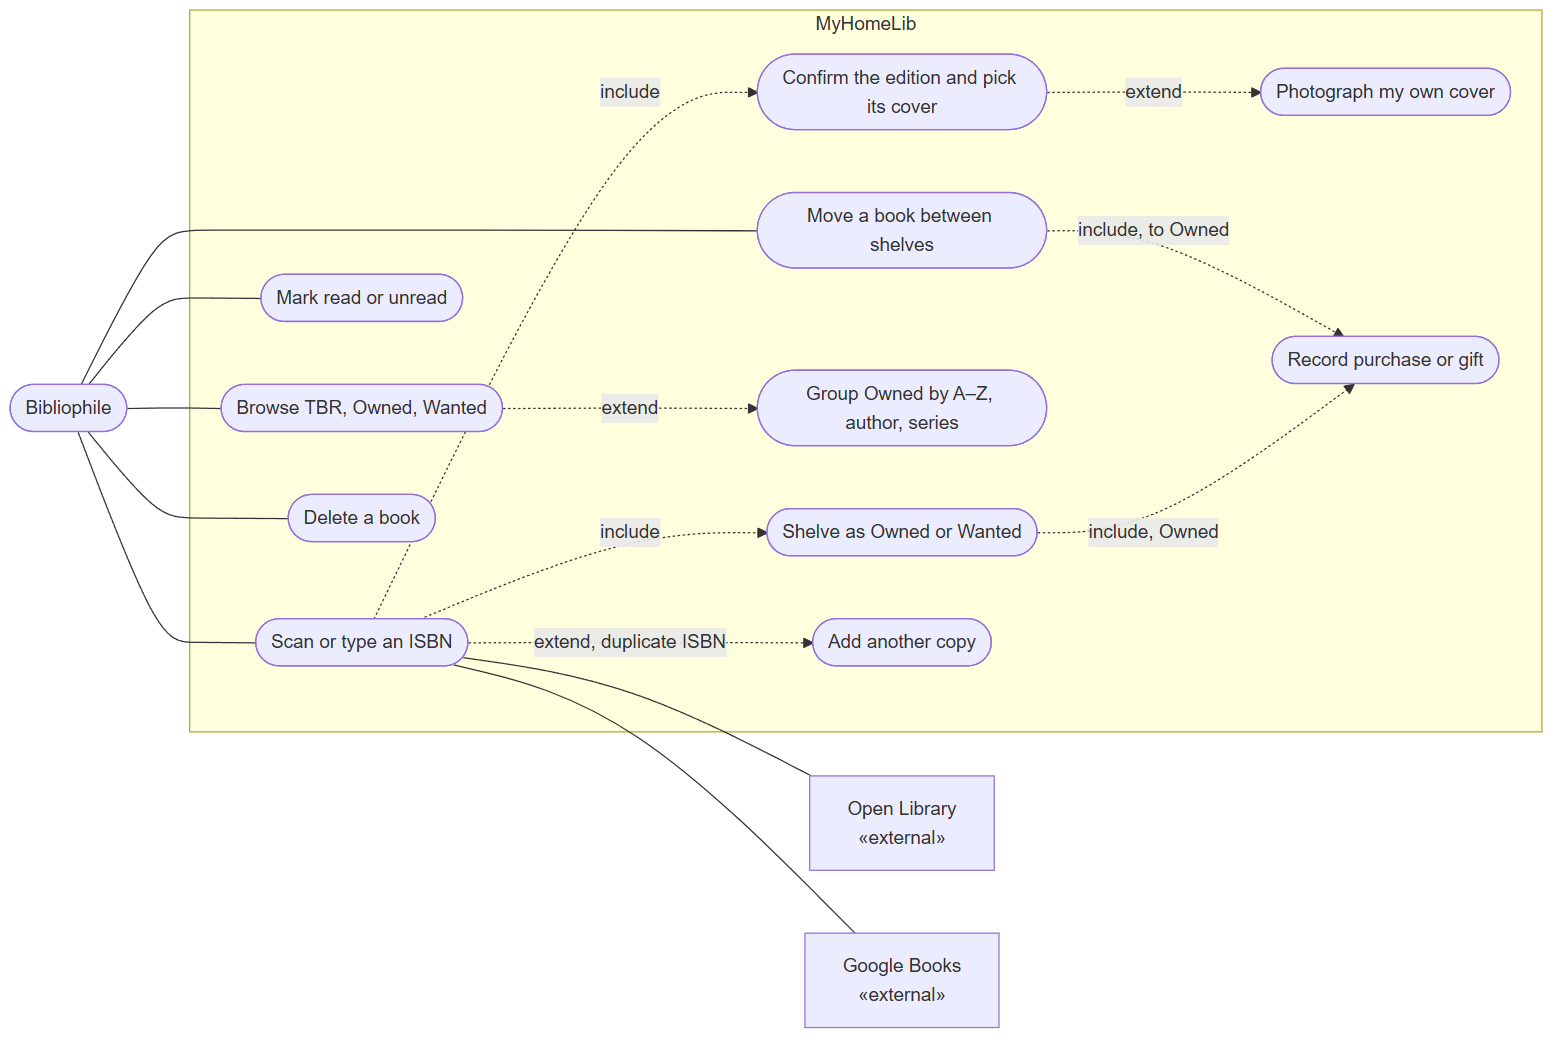
\includegraphics[width=\textwidth, height=0.48\textheight, keepaspectratio]{figures/use-case.png}
\caption{Use Case Diagram}
\label{fig:use_case}
\end{figure}

Figure~\ref{fig:use_case} shows what the bibliophile can do. Scanning \emph{includes} confirming the edition and choosing a shelf; choosing Owned \emph{includes} recording a purchase or gift. A duplicate ISBN \emph{extends} scanning into adding a copy. The two book sources are external actors of the scan use case.

\subsubsection{Activity Diagram}

\begin{figure}[htbp]
\centering
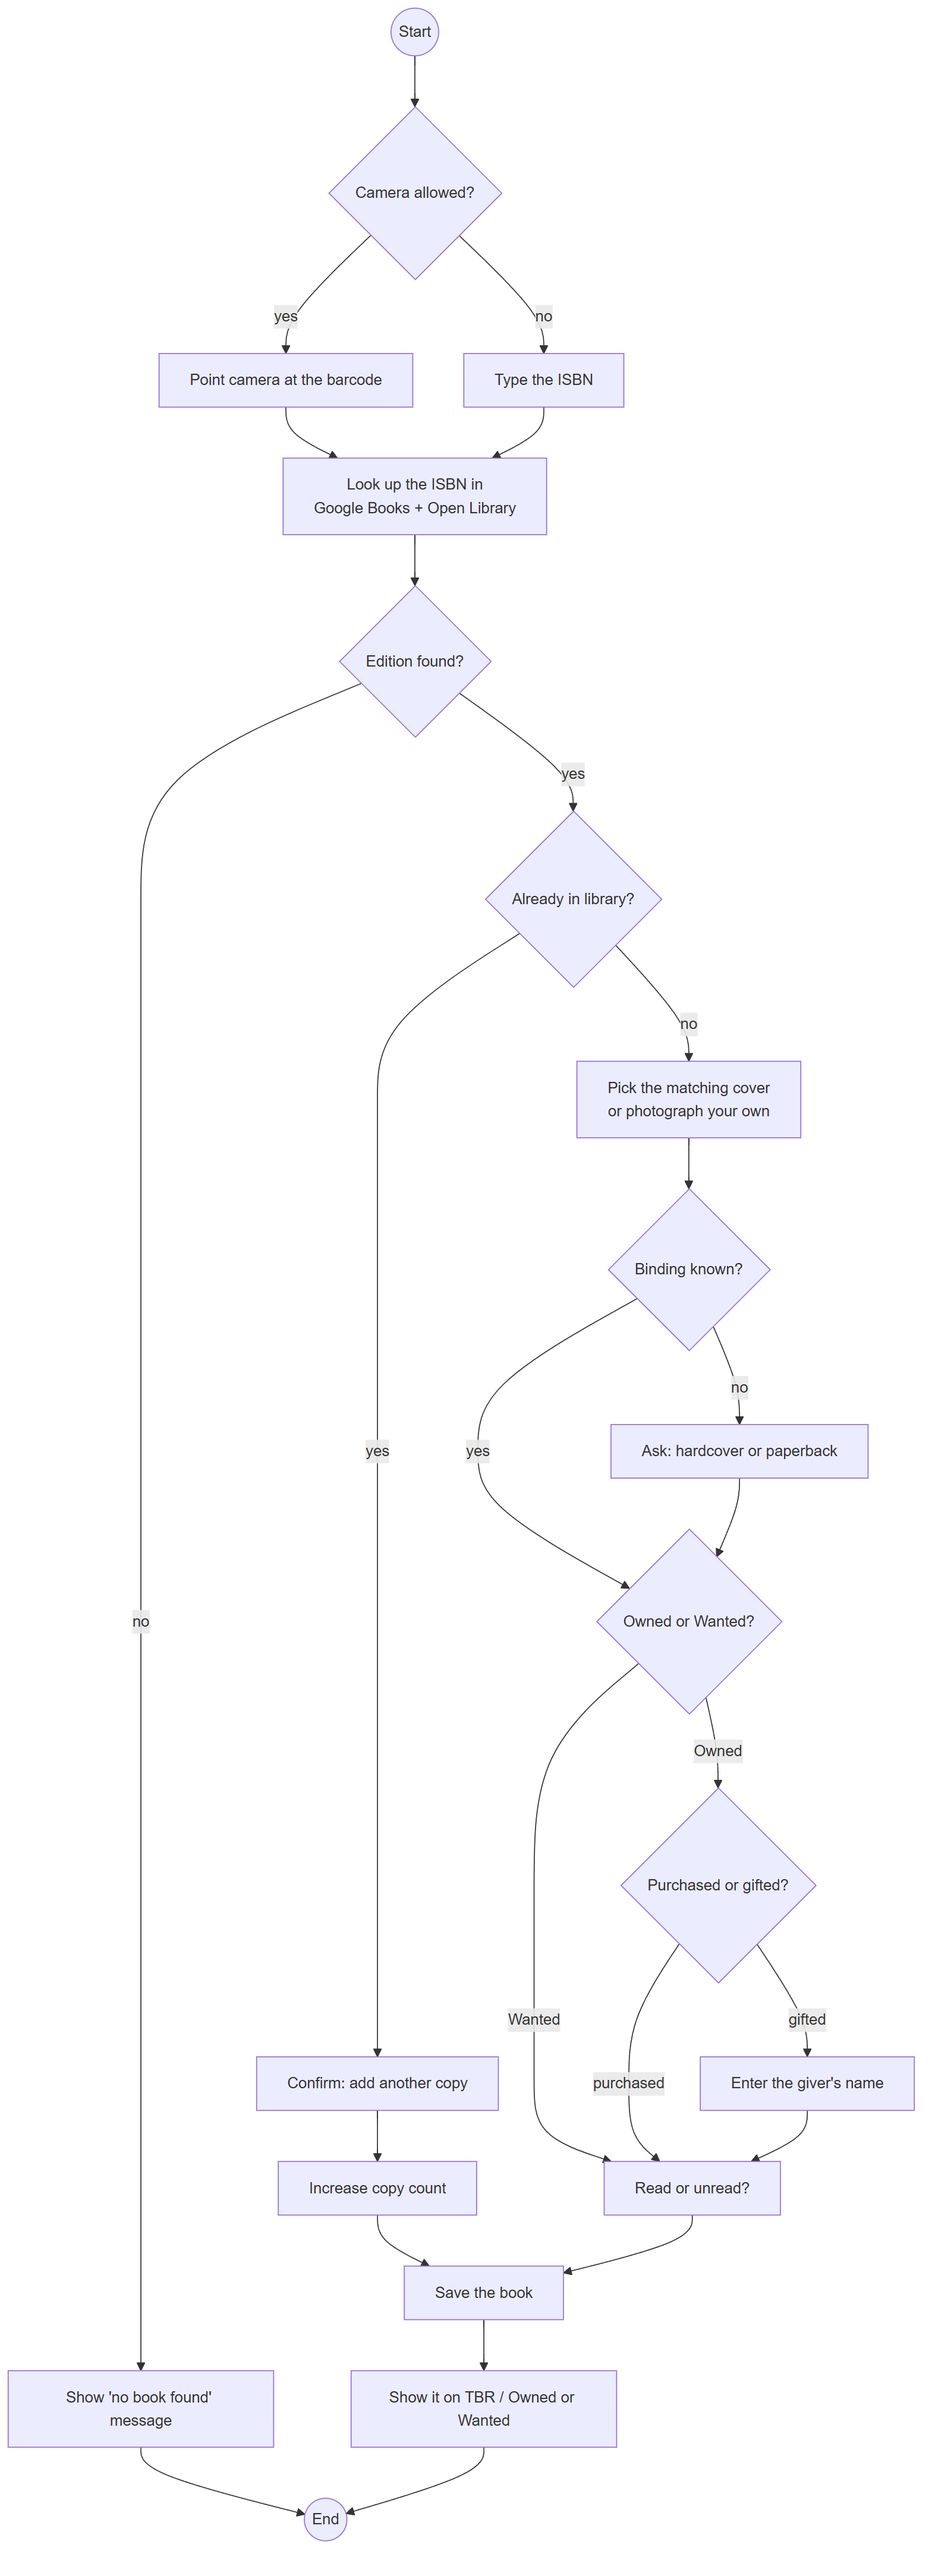
\includegraphics[width=\textwidth, height=0.8\textheight, keepaspectratio]{figures/activity-scan.png}
\caption{Activity Diagram: scanning a book}
\label{fig:activity}
\end{figure}

Figure~\ref{fig:activity} shows every decision in the scan flow, including the typed-ISBN fallback, the unknown-ISBN exit, the duplicate-copy shortcut, the optional binding question, and the gift branch.

\subsubsection{Class Diagram}

\begin{figure}[htbp]
\centering
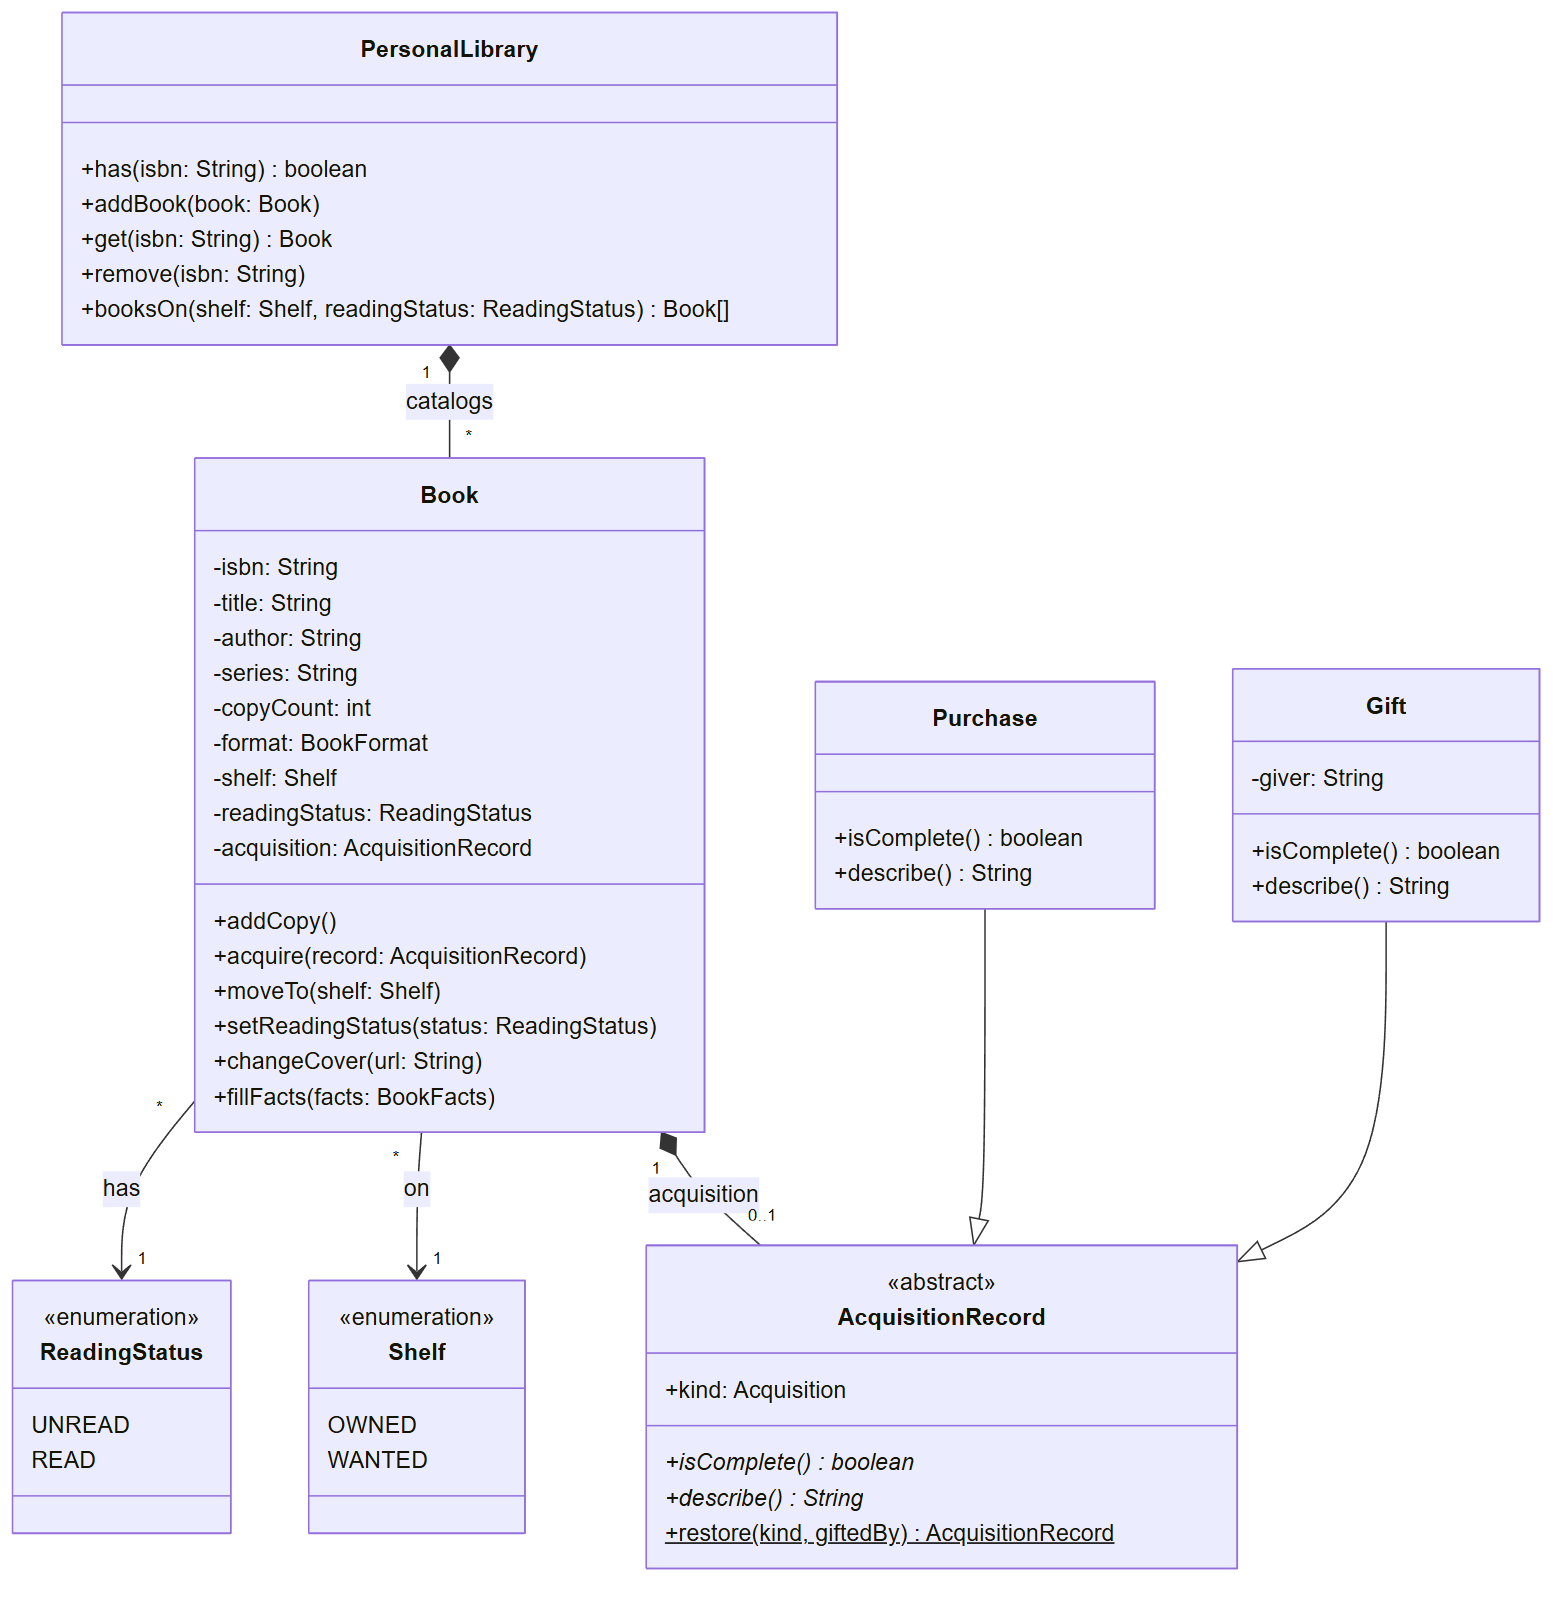
\includegraphics[width=\textwidth, height=0.58\textheight, keepaspectratio]{figures/class-domain.png}
\caption{Class Diagram: Domain model}
\label{fig:class_domain}
\end{figure}

\begin{figure}[htbp]
\centering
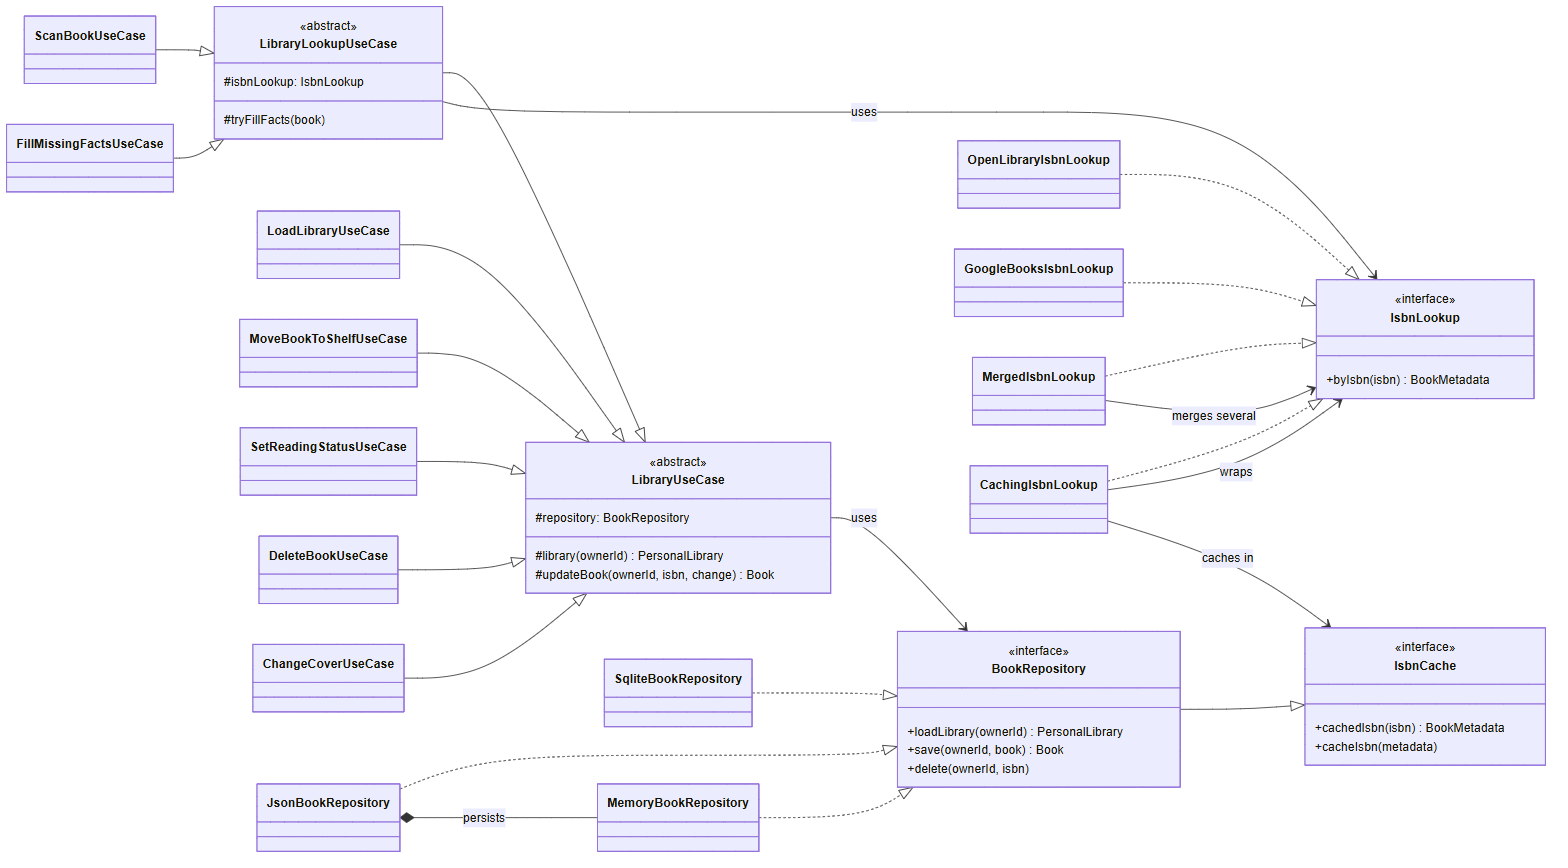
\includegraphics[width=\textwidth, height=0.55\textheight, keepaspectratio]{figures/class-service-data.png}
\caption{Class Diagram: Service use cases, ports, and Data adapters}
\label{fig:class_service}
\end{figure}

\begin{figure}[htbp]
\centering
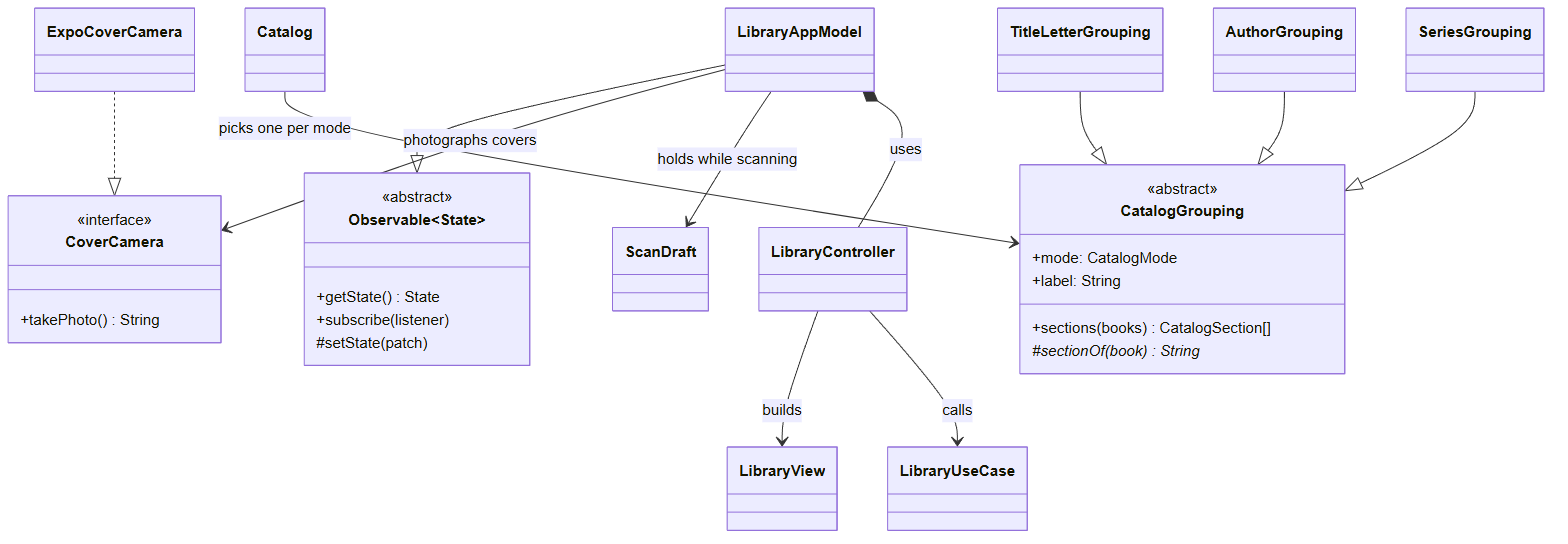
\includegraphics[width=\textwidth, height=0.4\textheight, keepaspectratio]{figures/class-presentation.png}
\caption{Class Diagram: Presentation view model and catalog strategies}
\label{fig:class_presentation}
\end{figure}


\FloatBarrier

Figures~\ref{fig:class_domain}, \ref{fig:class_service}, and~\ref{fig:class_presentation} show the classes. The object-oriented techniques used, and where:

\begin{longtable}{|L{3.6cm}|L{11cm}|}
\hline
\textbf{Technique} & \textbf{Where it is used} \\
\hline
\endhead
Encapsulation & \texttt{Book} keeps its state private; it changes only through rule-checking methods. \\
Abstract class + inheritance & \texttt{LibraryUseCase} $\rightarrow$ \texttt{LibraryLookupUseCase} $\rightarrow$ use cases; \texttt{AcquisitionRecord}; \texttt{CatalogGrouping}; \texttt{Observable}. \\
Polymorphism & \texttt{Purchase} and \texttt{Gift} answer \texttt{isComplete()} and \texttt{describe()} their own way. \\
Interfaces & \texttt{BookRepository}, \texttt{IsbnLookup}, \texttt{IsbnCache}, \texttt{CoverCamera}. \\
Composition & \texttt{PersonalLibrary} composes \texttt{Book}s; \texttt{JsonBookRepository} composes \texttt{MemoryBookRepository}. \\
Template Method & \texttt{LibraryUseCase.updateBook} (load $\rightarrow$ change $\rightarrow$ save). \\
Strategy & \texttt{TitleLetterGrouping}, \texttt{AuthorGrouping}, \texttt{SeriesGrouping}. \\
Decorator & \texttt{CachingIsbnLookup} and \texttt{MergedIsbnLookup} wrap other lookups. \\
Factory & \texttt{UseCases} builds every use case; \texttt{AcquisitionRecord.restore}. \\
Data Mapper & \texttt{BookRowMapper} is the only row $\leftrightarrow$ \texttt{Book} translation. \\
Observer / MVVM & \texttt{LibraryAppModel} extends \texttt{Observable}; React subscribes with \texttt{useObservable}. \\
Dependency injection & \texttt{CompositionRoot} passes adapters to the use cases; tests pass fakes. \\
\hline
\end{longtable}

\subsubsection{Sequence Diagram}

The sequence diagrams for scanning a book and for moving a Wanted book to Owned are shown in Figures~\ref{fig:sequence_scan} and~\ref{fig:sequence_move} (Section 4).

\FloatBarrier
\subsection{Rationale Management}

Rationale management records why each design decision was made. In this project every significant decision is recorded as an ADR in \texttt{docs/adr/}, so the reasoning stays next to the code and can be reviewed together with it.

\medskip
\noindent
\begin{tabular}{|L{1.2cm}|L{7.9cm}|L{5.0cm}|}
\hline
\textbf{ADR} & \textbf{Decision} & \textbf{Status} \\
\hline
001 & TypeScript + Expo Go modular monolith with four tier folders & Accepted (external-source line amended by 006) \\
002 & SQLite on the device, JSON fallback on the web, one port & Accepted \\
003 & Open Library for ISBN metadata (no key) & Accepted, amended by 006 \\
004 & No bookstore scraping & Accepted \\
005 & Expo Go instead of an app-store binary & Accepted \\
006 & Google Books as a second book source (optional key) & Accepted \\
007 & MVVM presentation with an observable view model & Accepted \\
008 & Design system: tokens, stylesheet imports, shared UI building blocks & Accepted \\
009 & Ports and adapters between Service and Data & Accepted \\
\hline
\end{tabular}

\subsubsection{Issues Addressed}

The first issue was \textbf{portability}: the review partner had to run the app without a Mac or paid accounts, which ruled out native builds and led to Expo Go. The second issue was \textbf{trustworthy data}: a catalog is only useful if it cannot contain duplicate entries or Owned books with no record of how they were acquired, so those rules had to live in the domain model where no screen can bypass them. The third issue was \textbf{matching the physical copy}: early testing showed that one ISBN can map to a wrong or missing cover, so the lookup had to become edition-first, consult a second source, and let the owner choose. The fourth issue was \textbf{keeping the code reviewable}: logic that had grown inside one large screen component had to move into classes that can be tested and diagrammed.

\subsubsection{Alternatives Considered}

\begin{itemize}
    \item \textbf{Native iOS app (Swift/Xcode)} or a \textbf{Flask web app}: rejected; the first needs a Mac, and the second is not a mobile app (ADR-001, ADR-005).
    \item \textbf{Scraping bookstore prices for the Wanted list}: rejected for reliability and terms-of-service reasons (ADR-004).
    \item \textbf{Open Library only}: simpler, but often wrong for a specific printing; Google Books was added as an optional second source (ADR-006).
    \item \textbf{Keeping screen logic in React hooks}: faster to write, but untestable without rendering and not class-based; replaced by an MVVM view model (ADR-007).
    \item \textbf{A UI component library}: would add dependencies and a generic look; a small token-based design system was built instead (ADR-008).
    \item \textbf{Plain JavaScript instead of TypeScript}: JavaScript is required by React Native, but it has no interfaces, abstract classes, or access modifiers, and it reports type mistakes only at run time. TypeScript was chosen because those features carry the course's object-oriented design straight into the code (the UML diagrams match the classes), the compiler refuses an adapter that does not implement its port, and all four tiers and the tests share one language.
    \item \textbf{Microservices or a backend server}: rejected; the library is private to one user and must work offline on a phone, so a server would add cost and failure points without benefit. A cloud store could later be added as one more \texttt{BookRepository} adapter.
\end{itemize}

\subsubsection{Decisions Made}

The design is centered on the scan workflow and the collection rules. The rules are methods of the domain classes; the use cases only orchestrate load, change, and save; the Data tier is replaceable behind two ports; and the screens are thin views of one observable view model. External sources are combined behind a single interface, so adding or removing a source does not change any caller.

\subsubsection{Criteria Used to Guide Decisions}

\begin{itemize}
    \item The design must satisfy the course constraints (portable platform, one store, no scraping, documented architecture).
    \item The diagrams must match the code, and automated tests must keep it that way.
    \item Each class must have one responsibility, and no logic may be written twice.
    \item The design must stay simple enough to finish in one semester and explain in a review.
\end{itemize}

\subsubsection{Design Debate and Final Resolution}

The main debate was between keeping the external integrations to the minimum (Open Library only) and matching the user's exact copy. Feedback from the instructor favored limiting integrations and removing scraping, while testing showed that a single free source produced wrong covers for many editions. The resolution was to add Google Books only through its official API, make its key optional so the app still runs without it, merge both sources behind the existing \texttt{IsbnLookup} port, and always let the owner choose or photograph the cover. This kept the architecture unchanged, respected the no-scraping rule, and met the user's need. A second debate concerned how much structure to add for the course's object-oriented requirements; the resolution was to introduce each pattern only where it removed real duplication or made a rule testable, and to document each one in the table above.

%==========================================================================
\section{Verification}
\label{sec:verification}

Verification in software is defined by the IEEE 1012 standard as ``the process of evaluating software to determine whether the products of a given development phase satisfy the conditions imposed at the start of that phase'' (IEEE, 2024).

MyHomeLib was verified in two complementary ways. First, \textbf{automated tests} (Jest) exercise every tier: 88 tests in 7 files, including tests that walk the view model through each user flow without any user interface, and tests that enforce the architecture rules. Second, each user story was \textbf{walked through in the running application}, and the screenshots below show the results. The numbered cases match the Test-Case column of the RTM.

\begin{table}[H]
\centering
\begin{tabular}{L{5cm} L{8cm} r}
\toprule
\textbf{Test file} & \textbf{What it verifies} & \textbf{Tests} \\
\midrule
domain.test.ts & Book and library rules: copies, acquisition, shelves, reading status & 17 \\
useCases.test.ts & Every use case against in-memory adapters & 23 \\
bookSources.test.ts & Open Library and Google Books parsing, merging, failures, caching & 16 \\
appModel.test.ts & Every user flow through the view model, no UI & 17 \\
controller.test.ts & Controller, library view, JSON round trip & 6 \\
catalog.test.ts & A--Z, author, and series grouping & 3 \\
architecture.test.ts & Tier dependency rules and stylesheet rules & 6 \\
\midrule
\textbf{Total} & \textbf{Test Suites: 7 passed; Tests: 88 passed} & \textbf{88} \\
\bottomrule
\end{tabular}
\caption{Automated test suite results (\texttt{npm test}, October 10, 2026)}
\label{tab:tests}
\end{table}

% ---------------- Sprint 4 ----------------
\subsection{Sprint 1 -- Project Proposal and Approval}

\begin{longtable}{L{0.4\linewidth} L{0.36\linewidth} L{0.14\linewidth}}
\toprule
\textbf{Process} & \textbf{Verification} & \textbf{Figure} \\
\midrule
\endhead
\textbf{(1)} We open the repository's README. It contains the approval paragraph, which names the platform (Expo Go on iOS and Android, with Expo web as a fallback), the core features, and the external book source. & Verify that the approval paragraph names the platform, features, and integration & README \\
\bottomrule
\end{longtable}

\subsection{Sprint 2 -- Tier Breakdown}

\begin{longtable}{L{0.4\linewidth} L{0.36\linewidth} L{0.14\linewidth}}
\toprule
\textbf{Process} & \textbf{Verification} & \textbf{Figure} \\
\midrule
\endhead
\textbf{(2)} We read the README's tier table. Each of Presentation, Service, Domain, and Data lists this system's own responsibilities, and each matches a top-level folder in the code. & Verify that each tier's real responsibilities are written down & Fig.~\ref{fig:system_architecture} \\
\bottomrule
\end{longtable}

\subsection{Sprint 3 -- C4 and UML Models}

\begin{longtable}{L{0.4\linewidth} L{0.36\linewidth} L{0.14\linewidth}}
\toprule
\textbf{Process} & \textbf{Verification} & \textbf{Figure} \\
\midrule
\endhead
\textbf{(3)} We open the README on GitHub. The C4 Context, Container, and Component diagrams and the UML class and sequence diagrams render from Mermaid, and the class names match the code (the architecture tests keep the tiers as drawn). & Verify that the C4 and UML diagrams exist, render, and match the code & Fig.~\ref{fig:context}, Fig.~\ref{fig:class_domain} \\
\bottomrule
\end{longtable}

\subsection{Sprint 4 -- Scanning, Shelves, and Copies}

\begin{longtable}{L{0.4\linewidth} L{0.36\linewidth} L{0.14\linewidth}}
\toprule
\textbf{Process} & \textbf{Verification} & \textbf{Figure} \\
\midrule
\endhead
\textbf{(4)} We open the app on the To be read tab with a small library. Owned unread books are listed; the switch shows the unread and read counts. & Verify that TBR lists Owned books split Unread / Read & Fig.~\ref{fig:v_tbr} \\
\textbf{(5)} We switch to Read. Only finished Owned books appear, marked with a leaf. With an empty library the shelf explains itself and offers Scan. & Verify that reading status is independent of the shelf & Fig.~\ref{fig:v_tbr} \\
\textbf{(6)} We open Owned and switch between A--Z, Author, and Series. Each grouping lists the same books under index headings. & Verify the three catalog groupings & Fig.~\ref{fig:gui_owned} \\
\textbf{(7)} In Series, the Dune series appears as a fan of covers with a count badge of 2; tapping it lists both books. & Verify series grouping and expansion & Fig.~\ref{fig:gui_owned} \\
\textbf{(8)} We scan the ISBN of Matilda, which is already cataloged. The popup says it is already in the library; confirming adds a copy, and the banner reports ``Copies: 2'' without a second entry. & Verify that a duplicate ISBN increments the copy count & Fig.~\ref{fig:v_duplicate} \\
\textbf{(9)} Repository tests save a library through browser (JSON) storage, reload it, and get the same books back, including a gift restored as a \texttt{Gift}; a cache test looks up the same ISBN twice and the book sources are asked only once. & Verify that the library persists and lookups are cached & Table~\ref{tab:tests} \\
\bottomrule
\end{longtable}

\begin{figure}[H]
    \centering
    \screen[0.18\textwidth]{tbr-unread}\hfill\screen[0.18\textwidth]{tbr-read}\hfill\screen[0.18\textwidth]{empty-tbr}
    \caption{TBR unread, TBR read, and the empty state}
    \label{fig:v_tbr}
\end{figure}


\begin{figure}[H]
    \centering
    \screen[0.18\textwidth]{duplicate-confirm}\hspace{1cm}\screen[0.18\textwidth]{duplicate-saved}
    \caption{A duplicate ISBN offers to add a copy (left); the copy count becomes 2 (right)}
    \label{fig:v_duplicate}
\end{figure}

% ---------------- Sprint 5 ----------------
\subsection{Sprint 5 -- Acquisition Rules}

\begin{longtable}{L{0.4\linewidth} L{0.36\linewidth} L{0.14\linewidth}}
\toprule
\textbf{Process} & \textbf{Verification} & \textbf{Figure} \\
\midrule
\endhead
\textbf{(10)} We open Beloved on the Wanted shelf and tap ``To Owned''. Before anything moves, the app asks whether it was purchased or gifted. & Verify that a Wanted book cannot move to Owned without a purchase or gift & Fig.~\ref{fig:v_move} \\
\textbf{(11)} We choose Gifted and tap Continue without a name. The popup stays open and nothing changes. & Verify that a gift requires the giver's name & Fig.~\ref{fig:v_move} \\
\textbf{(12)} We type the giver's name, continue, and answer Unread. The banner reports ``Moved to Owned (unread)'' and the book appears in Owned. & Verify that a complete gift moves the book & Fig.~\ref{fig:v_move_done} \\
\textbf{(13)} Domain tests try every move without an acquisition, with an empty giver, and with a blank giver; each is refused and the saved book stays Wanted. & Verify that a refused move saves nothing & Table~\ref{tab:tests} \\
\textbf{(14)} While scanning a new book we choose Owned; the app asks ``How did you get it?'' before the reading question. & Verify that scanning into Owned asks for the acquisition & Fig.~\ref{fig:v_scan2} \\
\bottomrule
\end{longtable}

\begin{figure}[H]
    \centering
    \screen[0.18\textwidth]{move-acquire}\hfill\screen[0.18\textwidth]{move-gift-name}\hfill\screen[0.18\textwidth]{move-gift-blank}
    \caption{Moving to Owned asks for the acquisition (left); a gift needs the giver's name (center, right)}
    \label{fig:v_move}
\end{figure}

\begin{figure}[H]
    \centering
    \screen[0.18\textwidth]{move-reading}\hspace{1cm}\screen[0.18\textwidth]{move-done}
    \caption{The last question is read or unread (left); the book moves to Owned (right)}
    \label{fig:v_move_done}
\end{figure}

% ---------------- Sprint 6 ----------------
\subsection{Sprint 6 -- Exact Edition, Refactor, and Design System}

\begin{longtable}{L{0.4\linewidth} L{0.36\linewidth} L{0.14\linewidth}}
\toprule
\textbf{Process} & \textbf{Verification} & \textbf{Figure} \\
\midrule
\endhead
\textbf{(15)} We open Scan. The camera preview shows the barcode target, and a typed-ISBN field is always available. & Verify the camera and the typed fallback & Fig.~\ref{fig:v_scan1} \\
\textbf{(16)} We type the ISBN of The Great Gatsby and look it up. The popup shows the edition (publisher, year) and saves nothing yet. & Verify that the lookup returns the edition and does not save & Fig.~\ref{fig:v_scan1} \\
\textbf{(17)} The popup offers every distinct cover the sources returned plus ``Your photo''. We tap the second cover; the check badge and the halo follow the choice. & Verify the cover picker & Fig.~\ref{fig:v_scan1} \\
\textbf{(18)} The sources did not state a binding, so the app asks ``Hardcover or paperback?''. A book whose binding is known skips this step (automated test). & Verify that the binding is asked only when unknown & Fig.~\ref{fig:v_scan2} \\
\textbf{(19)} We choose Owned, Purchased, and Unread. The banner reports ``Added The Great Gatsby to Owned (unread)''. & Verify that the scanned book is saved with every choice & Fig.~\ref{fig:v_scan3} \\
\textbf{(20)} We start another scan and tap ``Not this book''. The banner reports ``Nothing added'' and the library is unchanged. & Verify that cancelling a popup changes nothing & Fig.~\ref{fig:v_scan3} \\
\textbf{(21)} We look up an ISBN that no source knows. The banner reports ``No book found for ISBN \ldots''. & Verify the unknown-ISBN message & Fig.~\ref{fig:v_detail} \\
\textbf{(22)} Book-source tests feed recorded responses: edition data wins over work data, a different edition is never passed off as this one, every distinct cover is kept, and one source failing is tolerated. & Verify the edition-first merge & Table~\ref{tab:tests} \\
\textbf{(23)} View-model tests photograph a cover with a fake camera and check that the photo is saved; a refused camera explains itself and changes nothing. & Verify ``Your photo'' and camera refusal & Table~\ref{tab:tests} \\
\textbf{(24)} On a book's detail screen we tap ``Mark read''; the banner reports ``Marked read.'' and the book moves to the Read list. & Verify the read toggle & Fig.~\ref{fig:v_detail} \\
\textbf{(25)} We tap ``Delete from library''; a confirmation names the book and warns that every copy is removed. ``Keep it'' leaves it in place. & Verify that delete asks first & Fig.~\ref{fig:v_detail} \\
\textbf{(26)} The architecture tests read every source file: tiers depend only downward, no component defines a stylesheet or inline style, and only \texttt{App.tsx} reaches the composition root. All 6 pass. & Verify the tier and stylesheet rules & Table~\ref{tab:tests} \\
\textbf{(27)} We start the project with \texttt{npm start} and open it in Expo Go and in a web browser; no native build tools are required. & Verify the platform constraint & Fig.~\ref{fig:gui_tbr} \\
\textbf{(28)} Every text and background color pair was measured with the WCAG formula (lowest: 4.63:1, the danger button); cards announce ``title, by author, \ldots, read'' to screen readers; list entrances stop when Reduce Motion is on. & Verify accessibility & -- \\
\bottomrule
\end{longtable}

\begin{figure}[H]
    \centering
    \screen[0.18\textwidth]{scan}\hfill\screen[0.18\textwidth]{scan-confirm}\hfill\screen[0.18\textwidth]{scan-cover-picked}
    \caption{Scan screen (left); the edition with its covers (center); choosing the second cover (right)}
    \label{fig:v_scan1}
\end{figure}

\begin{figure}[H]
    \centering
    \screen[0.18\textwidth]{scan-binding}\hfill\screen[0.18\textwidth]{scan-shelf}\hfill\screen[0.18\textwidth]{scan-acquire}
    \caption{Binding question (left), shelf choice (center), and acquisition for Owned (right)}
    \label{fig:v_scan2}
\end{figure}

\begin{figure}[H]
    \centering
    \screen[0.18\textwidth]{scan-reading}\hfill\screen[0.18\textwidth]{scan-saved}\hfill\screen[0.18\textwidth]{scan-cancelled}
    \caption{Reading question (left); the book is added (center); a cancelled scan adds nothing (right)}
    \label{fig:v_scan3}
\end{figure}

\begin{figure}[H]
    \centering
    \screen[0.18\textwidth]{mark-read}\hfill\screen[0.18\textwidth]{delete-confirm}\hfill\screen[0.18\textwidth]{unknown-isbn}
    \caption{Marked read (left); delete confirmation (center); an unknown ISBN (right)}
    \label{fig:v_detail}
\end{figure}

%==========================================================================
\section{References}

\begin{itemize}[leftmargin=0.5in, itemindent=-0.5in, labelsep=0in]
\item Anthropic. (2026). \textit{Claude} (Opus 5.5 model) [Large language model], accessed through \textit{Claude Code} [Computer software]. Retrieved from \url{https://www.anthropic.com/claude-code}
\item Brown, S. (n.d.). \textit{The C4 model for visualising software architecture}. Retrieved from \url{https://c4model.com/}
\item Expo. (n.d.). \textit{Expo documentation}. Retrieved from \url{https://docs.expo.dev/}
\item Gamma, E., Helm, R., Johnson, R., \& Vlissides, J. (1994). \textit{Design patterns: Elements of reusable object-oriented software}. Addison-Wesley.
\item Google. (n.d.). \textit{Books API}. Retrieved from \url{https://developers.google.com/books}
\item Institute of Electrical and Electronics Engineers. (2024). \textit{IEEE standard for system, software, and hardware verification and validation} (IEEE Std 1012-2024). IEEE.
\item Internet Archive. (n.d.). \textit{Open Library APIs}. Retrieved from \url{https://openlibrary.org/developers/api}
\item Martin, R. C. (2017). \textit{Clean architecture: A craftsman's guide to software structure and design}. Prentice Hall.
\item Nygard, M. (2011). \textit{Documenting architecture decisions}. Retrieved from \url{https://cognitect.com/blog/2011/11/15/documenting-architecture-decisions}
\item Sommerville, I. (2021). \textit{Software engineering} (10th ed.). Pearson.
\item World Wide Web Consortium. (2023). \textit{Web Content Accessibility Guidelines (WCAG) 2.2}. Retrieved from \url{https://www.w3.org/TR/WCAG22/}
\end{itemize}

\end{document}
